% !TeX root = main.tex
\chapterimage{chapter-08-scratch.jpg}
\chapter{Programmazione creativa con Scratch}\label{capitolo-8-programmazione-creativa-con-scratch}

Dopo le attività unplugged e l'uso di ambienti guidati come Code.org, \textbf{Scratch rappresenta il successivo passo naturale per introdurre gli alunni e le alunne alla programmazione.} Si tratta di un ambiente gratuito, progettato per permettere di esprimere le proprie idee attraverso l'informatica, costruendo giochi, animazioni e storie interattive mediante un linguaggio a blocchi semplice e intuitivo. Sviluppato dal gruppo Lifelong Kindergarten del MIT Media Lab e \textbf{ispirato alla teoria costruzionista dell'apprendimento}, Scratch offre un contesto di programmazione accessibile e ricco di possibilità. Come su Code.org, le istruzioni sono presentate sotto forma di blocchi colorati che si incastrano tra loro, eliminando le difficoltà legate alla sintassi e permettendo alle alunne e agli alunni di concentrarsi sulla logica, sulla progettazione e sulla creatività.

La filosofia educativa alla base di Scratch si riassume nelle ``4 P'': \textbf{Peers}, la collaborazione tra pari; \textbf{Projects}, l'apprendimento orientato a un progetto significativo; \textbf{Passion}, il coltivare interessi autentici; e \textbf{Play}, il valore del gioco come spazio di esplorazione \parencite{resnick-2018}. Ed è proprio questa filosofia a segnare la differenza principale rispetto ad ambienti più strutturati e sequenziali come Code.org: mentre questi ultimi guidano gli alunni e le alunne attraverso percorsi molto guidati, Scratch offre uno spazio aperto in cui esplorare, sperimentare e costruire in autonomia. Questa libertà progettuale consente di mettere in gioco le proprie idee, provare soluzioni alternative e sviluppare competenze creative e collaborative che vanno oltre la semplice risoluzione di esercizi.

Sebbene non sia l'unico strumento disponibile per introdurre la programmazione a scuola, Scratch è uno dei pochi ambienti progettati in modo pedagogicamente solido per le fasce d'età che vanno dalla primaria ai primi anni di secondaria di secondo grado. È gratuito, accessibile da diversi dispositivi e nasce esplicitamente per supportare percorsi educativi basati sulla creatività, sulla collaborazione e sull'apprendimento attivo. Il suo design user-friendly lo rende adatto non solo agli alunni e alunne, ma anche a docenti e genitori che desiderano accompagnarli nelle attività. La versatilità dell'ambiente permette di utilizzarlo sia in contesti didattici sia in situazioni ricreative, poiché si adatta con facilità a diverse finalità e livelli di esperienza.

La combinazione di semplicità e potenzialità è uno dei motivi principali per cui Scratch è così diffuso: è possibile iniziare con progetti essenziali, come piccole animazioni o giochi molto semplici, e sviluppare progressivamente competenze più avanzate, esplorando concetti di logica, progettazione e pensiero computazionale in modo naturale e graduale. \textbf{Questa progressione fluida non è casuale}, ma riflette alcune scelte di design fondamentali, riassumibili in tre principi chiave \parencite{resnick-2018}:

\begin{itemize}
\item
  \textbf{Low floor} (pavimento basso): l'ambiente è facile da approcciare e permette di ottenere risultati soddisfacenti fin dai primi tentativi, grazie anche all'interfaccia grafica intuitiva.
\item
  \textbf{High ceiling} (soffitto alto): una volta acquisite le basi, è possibile realizzare progetti sempre più complessi, aumentando gradualmente le proprie competenze.
\item
  \textbf{Wide walls} (pareti ampie): lo stesso ambiente può essere utilizzato per creare progetti molto diversi tra loro (ad esempio giochi, storie, animazioni, arte interattiva, quiz\ldots), favorendo la creatività, la sperimentazione e la produzione di artefatti originali.
\end{itemize}

\section{Prerequisiti }\label{prerequisiti-5}

Le attività di questo capitolo sono veramente efficaci se alunni e alunne hanno già avuto qualche esperienza di base con i concetti informatici affrontati nei capitoli precedenti, in particolare nelle attività dedicate alla programmazione visuale di Code.org. Avere già familiarità con idee come \emph{sequenza di istruzioni}, \emph{movimento di un personaggio} e \emph{ripetizione} aiuta a comprendere più rapidamente il funzionamento dei blocchi di Scratch per poter sviluppare progetti più ricchi.

\section{Traguardi e obiettivi generali }\label{traguardi-e-obiettivi-generali-5}

\begin{itemize}
\item
  Orientarsi nell'ambiente di programmazione Scratch (stage, sprite, Area dei blocchi, Area del codice), riuscendo a selezionare personaggi e sfondi e ad avviare l'esecuzione di un programma.
\item
  Creare programmi in sequenza, disponendo i blocchi in un ordine logico per far compiere azioni a un personaggio.
\item
  Utilizzare le ripetizioni per eseguire più volte una stessa istruzione o sequenza di istruzioni, rendendo i programmi più compatti.
\item
  Utilizzare in modo consapevole le istruzioni di movimento per controllare posizione, direzione e spostamenti degli sprite.
\item
  Sincronizzare le azioni di più sprite, gestendo dialoghi e turni di parola mediante attese temporizzate.
\item
  Sperimentare la strategia di prova ed errore, osservando il comportamento dello sprite, interpretando i feedback dell'ambiente ed effettuando correzioni (debugging) per migliorare il programma.
\item
  Progettare e realizzare piccole animazioni o storie, combinando sprite, costumi, sfondi e blocchi di codice per dare forma a idee personali.
\end{itemize}

\section{Preparazione }\label{preparazione-8}

L'accesso alla piattaforma di Scratch è completamente libero, gratuito e immediato. È possibile utilizzare Scratch:

\begin{itemize}
\item
  \textbf{online}, all'indirizzo \urloriginale{https://scratch.mit.edu/};
\item
  \textbf{offline}, scaricando Scratch App (gratuita per Windows, Mac, ChromeOS e Android) all'indirizzo \urloriginale{https://scratch.mit.edu/download}.
\end{itemize}

Sul sito ufficiale sono disponibili una vasta documentazione, una community internazionale e numerose risorse didattiche pensate appositamente per la scuola.

\subsection{Iscrizione dell'insegnante e della classe a Scratch }\label{iscrizione-dellinsegnante-e-della-classe-a-scratch}

Per utilizzare Scratch, è possibile utilizzare un account normale oppure un \textbf{account docente}, che permette di creare le proprie classi come in Code.org. A differenza degli account normali che sono attivi da subito, gli account docente richiedono circa 24 ore per essere approvati. Per registrare un account docente:

\begin{enumerate}
\def\labelenumi{\arabic{enumi}.}
\item
  visita \linkbreve{scratchDocenti};
\item
  seleziona ``Richiedi un account docente'';
\item
  compila il breve modulo con i tuoi dati;
\item
  conferma la registrazione tramite il link ricevuto via e-mail.
\end{enumerate}

L'\textbf{account docente} di Scratch permette di creare e gestire classi, creare account per alunni e alunne senza richiedere i loro indirizzi e-mail, reimpostarne le password e organizzare i progetti condivisi in gallerie. Consente inoltre di monitorare i commenti degli studenti e delle studentesse e di intervenire eliminando commenti o ritirando dalla condivisione singoli progetti. Facilita così l'organizzazione e la supervisione del lavoro in classe\footnote{Nota bene: non crea uno spazio privato né permette di impedire agli studenti di condividere i propri progetti.}. Ulteriori informazioni sono disponibili nella guida ufficiale (in inglese): \linkbreve{guidaAccountDocente}.


\subsection{E se non vogliamo creare nessun account?}


Esattamente come in Code.org, è possibile utilizzare Scratch anche \textbf{senza effettuare l'accesso}. In questo caso:

\begin{itemize}
\item
  i progetti possono comunque essere creati;
\item
  ma \textbf{non verranno salvati} online o nella classe; è tuttavia possibile scaricarli come file locali. Per attività singole (es. esercitazioni brevi), questa soluzione è pienamente utilizzabile. Basta accedere al sito di Scratch (\urloriginale{https://scratch.mit.edu/}) e cliccare su \textbf{Crea}.
\end{itemize}

\section{Attività 1: benvenuti in Scratch!}

\ruoliattivita{\ruoloProgrammatore}

In questa prima attività è importante illustrare agli alunni e alle alunne le aree dell'interfaccia.


\begin{consiglio}[Maestr* si è buggato... è tutto in inglese!]

Scratch può essere un valido alleato per l'inclusione di chi non è italofono.

L'ambiente Scratch è infatti disponibile in circa 70 lingue: questo permette a ciascuno di lavorare nella lingua che conosce meglio, riducendo il carico cognitivo e favorendo la comprensione delle attività.

\begin{center}
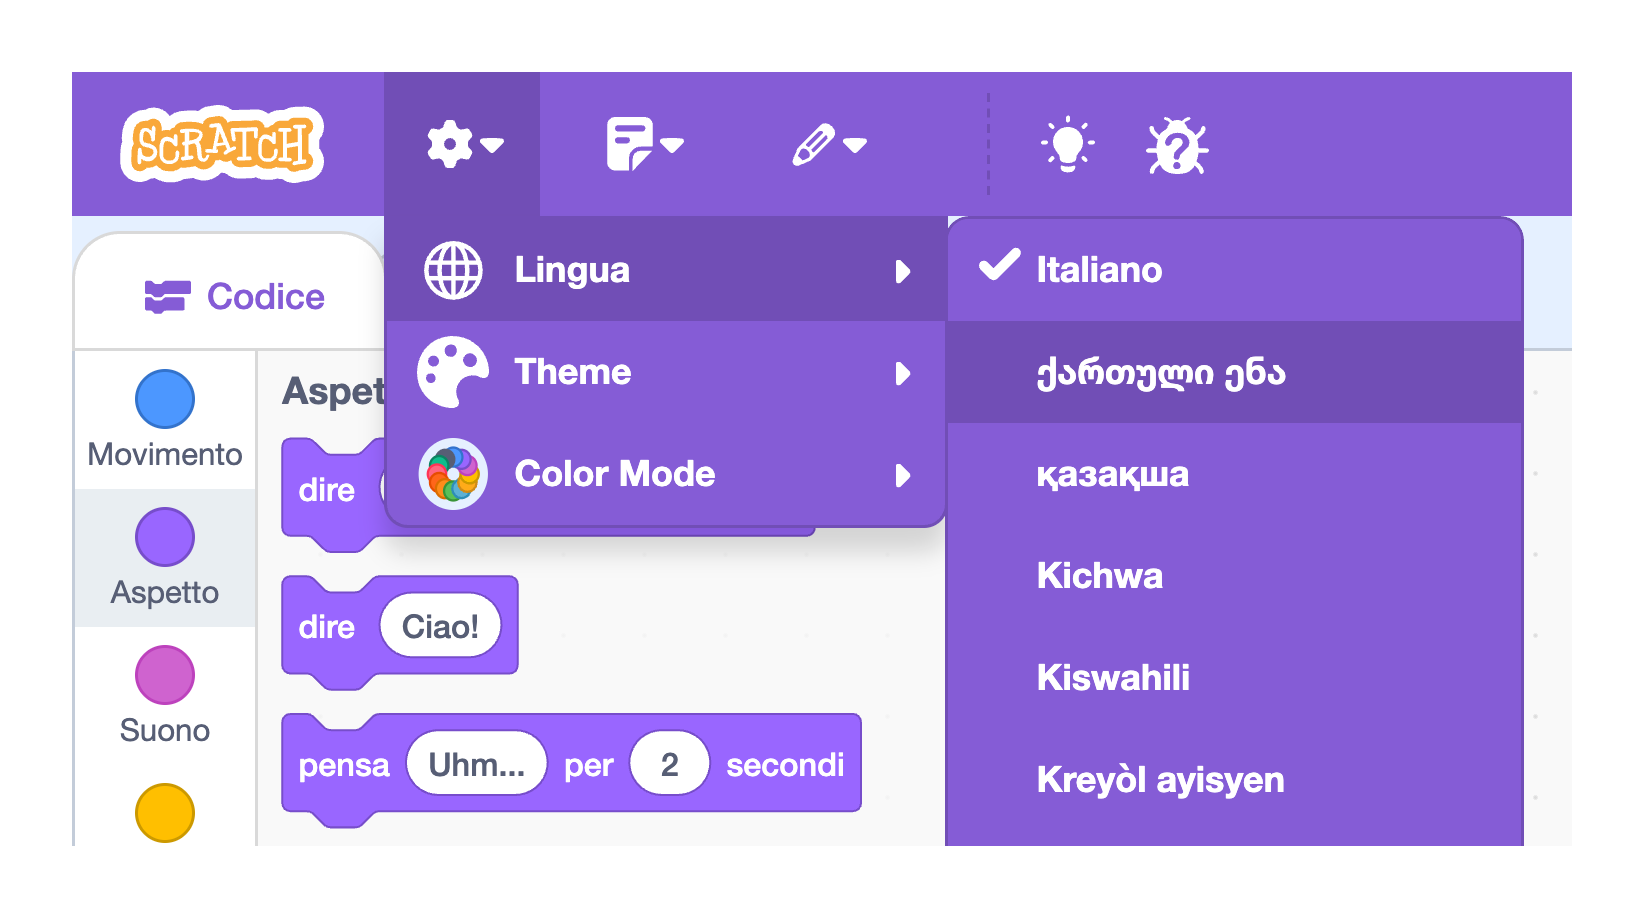
\includegraphics[trim=72bp 72bp 72bp 72bp,clip,width=0.65\linewidth]{img/scratch-lingua.png}\label{credito:scratch-lingua-1}
\end{center}
\newpage

Per modificare la lingua è sufficiente aprire il menu \textbf{Impostazioni} ➜ \textbf{Lingua} e selezionare l'opzione desiderata. L'interfaccia si aggiornerà immediatamente, rendendo i blocchi e i comandi più accessibili e consentendo ai bambini di partecipare con maggiore sicurezza alle attività di programmazione.

Dal menu Impostazioni è possibile scegliere anche colori ad elevato contrasto per facilitare la distinzione dei blocchi.

\end{consiglio}

Ecco come appare la finestra di Scratch dopo averla aperta sul proprio pc.

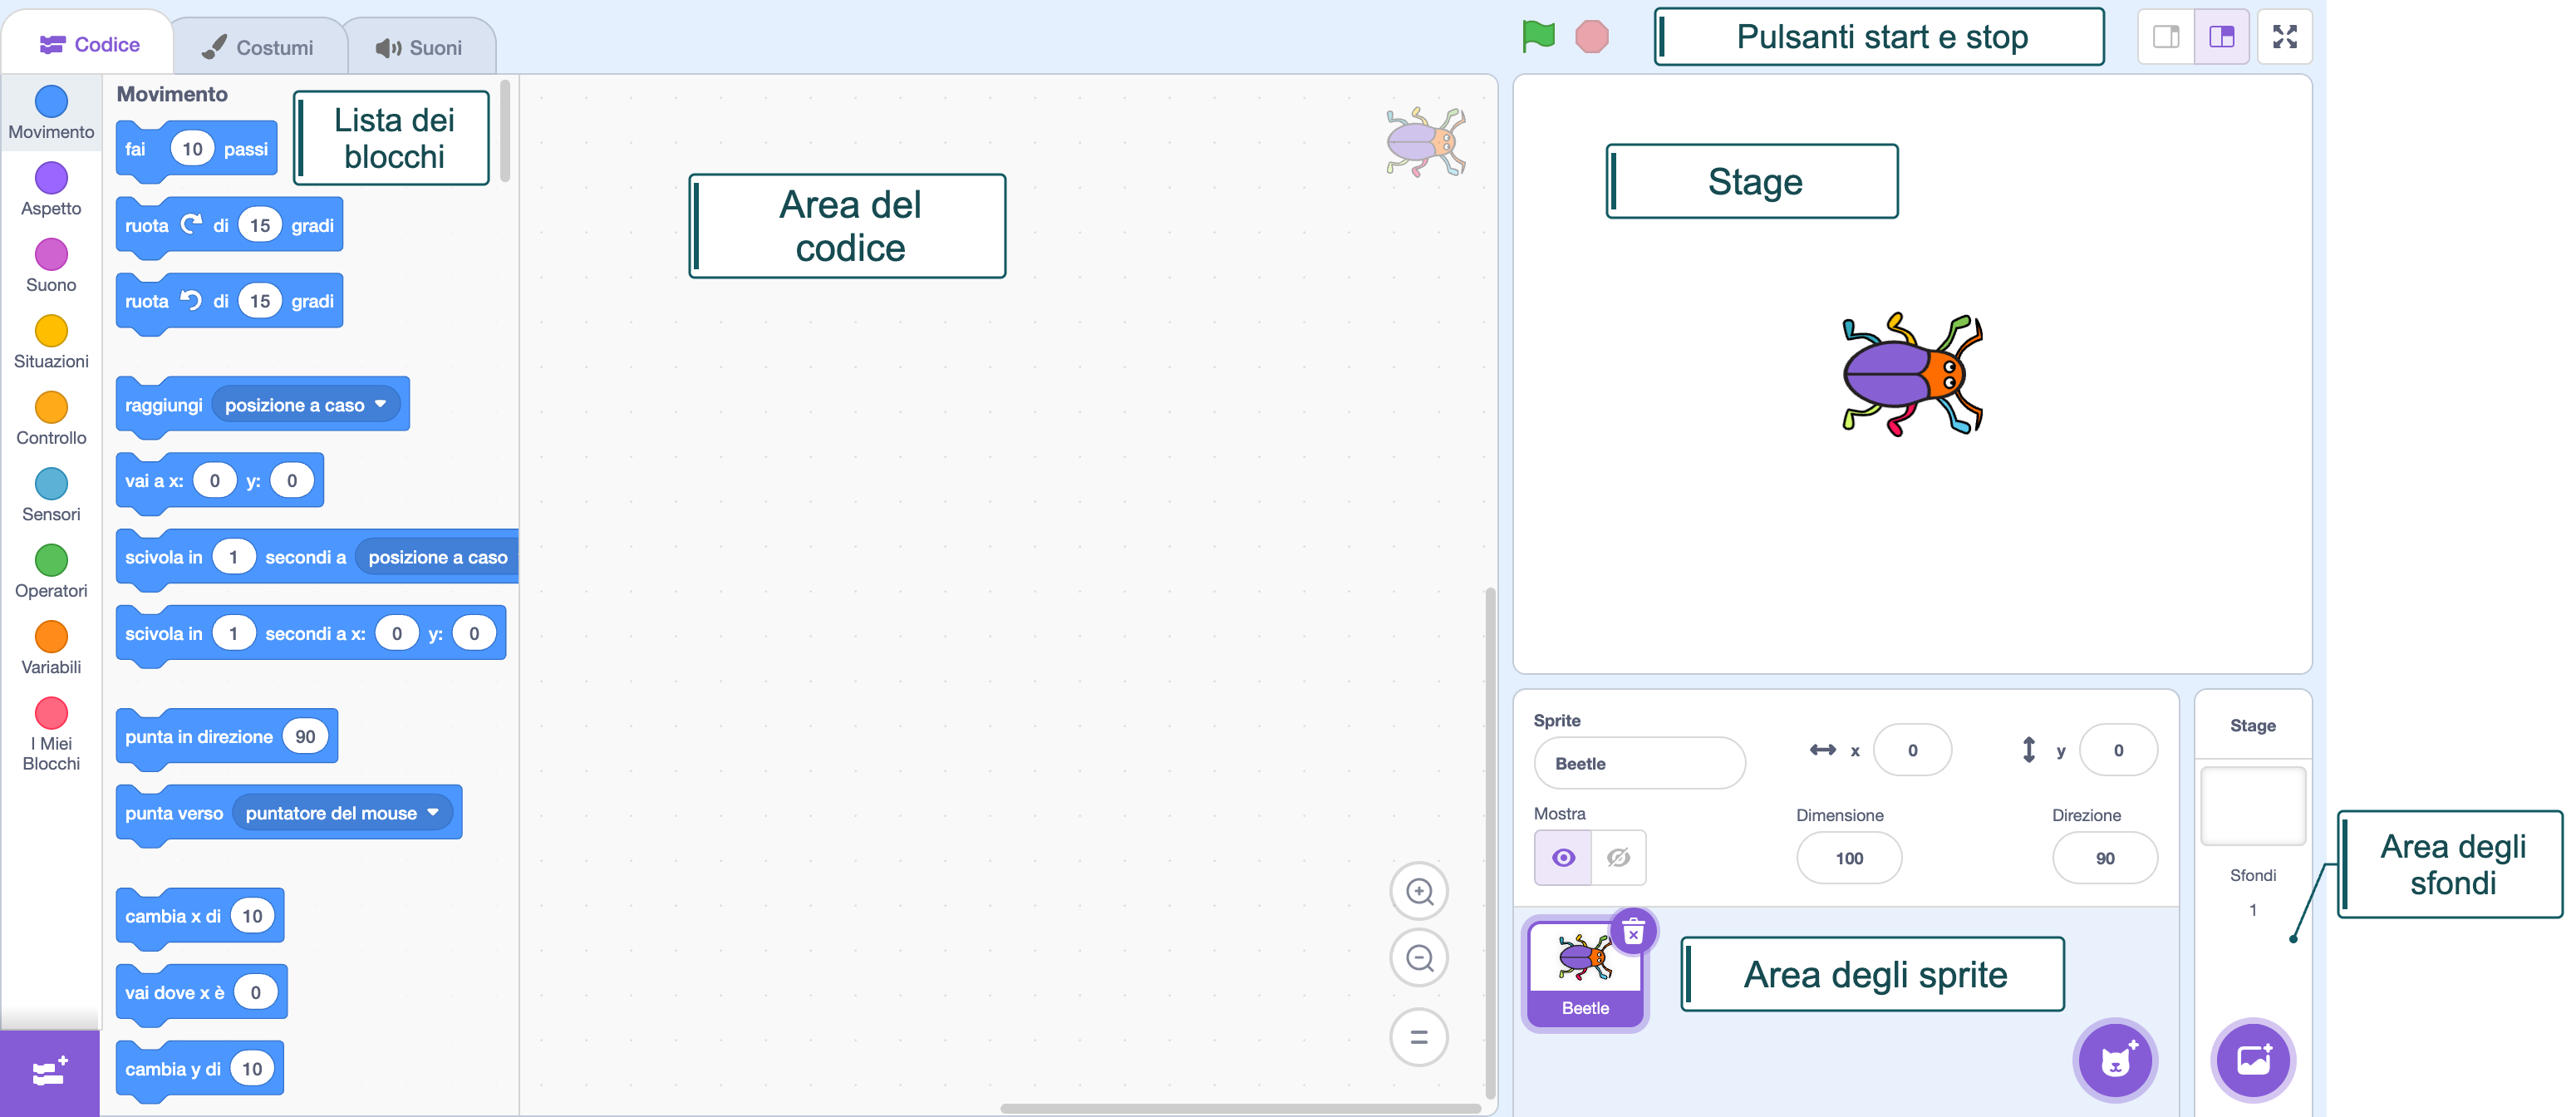
\includegraphics[width=\linewidth]{img/scratch-interfaccia.png}\label{credito:scratch-interfaccia-1}

L'interfaccia di Scratch è organizzata in aree ben distinte, pensate per aiutare gli alunni e le alunne a costruire i propri progetti in modo semplice e intuitivo. Nell'immagine sono visibili le principali aree dell'interfaccia: Lista dei blocchi, Area del codice, stage, Aree degli sprite e degli sfondi. Comprendere la funzione di ciascuna parte è fondamentale per accompagnare alunni e alunne nei primi passi della programmazione.

\begin{itemize}
\item
  \textbf{Lista dei blocchi} (a sinistra)\textbf{:} l'elenco dei blocchi disponibili, come quello presente nei Manuali delle istruzioni, divisi per categorie e riconoscibili grazie al codice colore.
\item
  \textbf{Area del codice} (al centro): lo spazio per costruire i programmi, trascinando nell'area i blocchi presi dalla lista dei blocchi e incastrandoli tra loro. Ogni personaggio (chiamato \textbf{sprite}) avrà il \textbf{proprio codice}: quando si seleziona uno sprite, l'Area del codice mostra quello relativo a quel personaggio.
\item
  \textbf{Stage} (in alto a destra): la scena in cui si svolge l'animazione o il gioco che si sta costruendo. Nello stage si vedono i personaggi in movimento, gli sfondi scelti e gli effetti delle azioni che hanno programmato. In alto compaiono anche i \textbf{pulsanti start} (bandierina verde) e \textbf{stop} (cartello stradale rosso).
\item
  \textbf{Area degli sprite} (in basso a destra): qui sono mostrati gli sprite presenti nel progetto, lo sprite selezionato in quel momento (con il contorno azzurro) e le proprietà dello sprite selezionato (posizione con coordinate x e y, direzione, visibilità, dimensione). Da qui è possibile aggiungere nuovi sprite, cancellarli e duplicarli.
\item
  \textbf{Area degli sfondi} (accanto all'Area degli sprite), dove è possibile cambiare o aggiungere sfondi allo stage.
\end{itemize}


In sintesi, l'immagine mostra \textbf{dove si trovano i blocchi} (colonna sinistra), \textbf{dove si costruisce il programma} (zona centrale), \textbf{dove si vede il risultato} (lo stage in alto a destra), \textbf{dove si gestiscono i personaggi} e \textbf{gli sfondi} (in basso a destra).

\section{Attività 2: diventa un regista con Scratch!}

\ruoliattivita{\ruoloProgrammatore}


In questa attività viene chiesto a bambini e bambine di diventare registi creando un'animazione con un dialogo, in cui il nostro personaggio potrà parlare tramite fumetti.

Prima di lavorare sul codice, vediamo come inserire uno sprite e uno sfondo. Per creare un \textbf{nuovo sprite} bisogna premere sull'icona con la faccia del gatto e scegliere uno dei modi possibili (dall'alto verso il basso):

\noindent
\begin{minipage}[c]{0.81\linewidth}
\begin{itemize}
\item
  caricare un file;
\item
  farlo scegliere a Scratch in maniera casuale;
\item
  disegnarlo;
\item
  sceglierlo dalla libreria di Scratch.
\end{itemize}
\end{minipage}\hfill
\begin{minipage}[c]{0.15\linewidth}
\centering
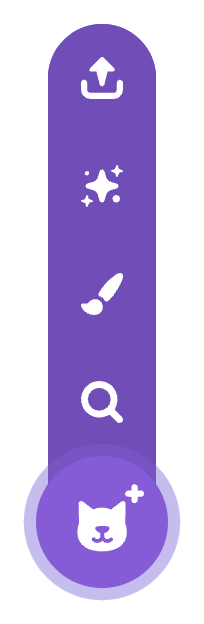
\includegraphics[height=3.8cm]{img/scratch-menu-sprite.png}\label{credito:scratch-menu-sprite-1}
\end{minipage}
\par

Per creare un \textbf{nuovo sfondo} bisogna premere sull'icona in basso a destra dello schermo e scegliere uno dei modi possibili (dall'alto verso il basso):

\noindent
\begin{minipage}[c]{0.81\linewidth}
\begin{itemize}
\item
  caricare un file;
\item
  farlo scegliere a Scratch in maniera casuale;
\item
  disegnarlo;
\item
  sceglierlo dalla libreria di Scratch.
\end{itemize}
\end{minipage}\hfill
\begin{minipage}[c]{0.15\linewidth}
\centering
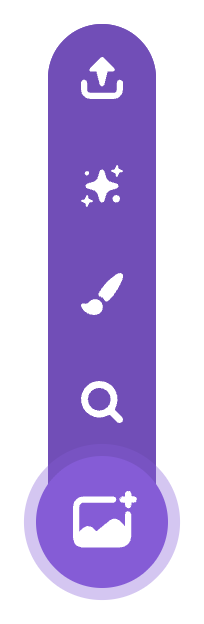
\includegraphics[height=3.8cm]{img/scratch-menu-sfondo.png}\label{credito:scratch-menu-sfondo-1}
\end{minipage}
\par


\subsection{E ora, crea il codice!}


Un programma è composto da una serie di blocchi colorati (tra quelli disponibili nella lista dei blocchi, a sinistra dello schermo) agganciati sequenzialmente uno sotto l'altro.

In Scratch ogni blocco ha un colore che identifica la categoria di comandi a cui appartiene: questo aiuta alunni e alunne a riconoscerne rapidamente la funzione e, con il tempo, a intuire che cosa fa un blocco ancora prima di usarlo; puoi decidere se presentarli passo passo oppure lasciare che li esplorino liberamente, sfruttando proprio il colore come guida pratica.

\begin{itemize}
\item
  \textbf{Movimento} (blu): istruzioni che fanno muovere lo sprite sulla scena.
\item
  \textbf{Aspetto} (viola): istruzioni per far ``parlare'' e ``pensare'' uno sprite (con il meccanismo dei fumetti, quindi visualizzando del testo) e per cambiare il suo aspetto.
\item
  \textbf{Suono} (rosa): istruzioni per riprodurre dei suoni.
\item
  \textbf{Situazioni} (giallo): istruzioni per avviare una sequenza di istruzioni come reazione ad un evento, come il click sulla bandierina verde o la pressione di un tasto.
\item
  \textbf{Controllo} (arancione): istruzioni che gestiscono il flusso del programma, permettendo di ripetere azioni, prendere decisioni, attendere, fermare l'esecuzione.
\item
  \textbf{Sensori} (azzurro): istruzioni che permettono allo sprite di ottenere informazioni dall'ambiente (per esempio posizione del mouse, tasti premuti o contatto con altri oggetti) e usarle per guidare il comportamento del programma.
\item
  \textbf{Operatori} (verde): istruzioni per eseguire operazioni aritmetiche, operazioni logiche (cioè verifiche di tipo vero/falso utili a decidere come far agire lo sprite) e per lavorare con i testi.
\item
  \textbf{Variabili e liste} (arancione chiaro): istruzioni per memorizzare informazioni e riutilizzarle nel programma, ad esempio per salvare il punteggio di un gioco.
\end{itemize}

\begin{center}
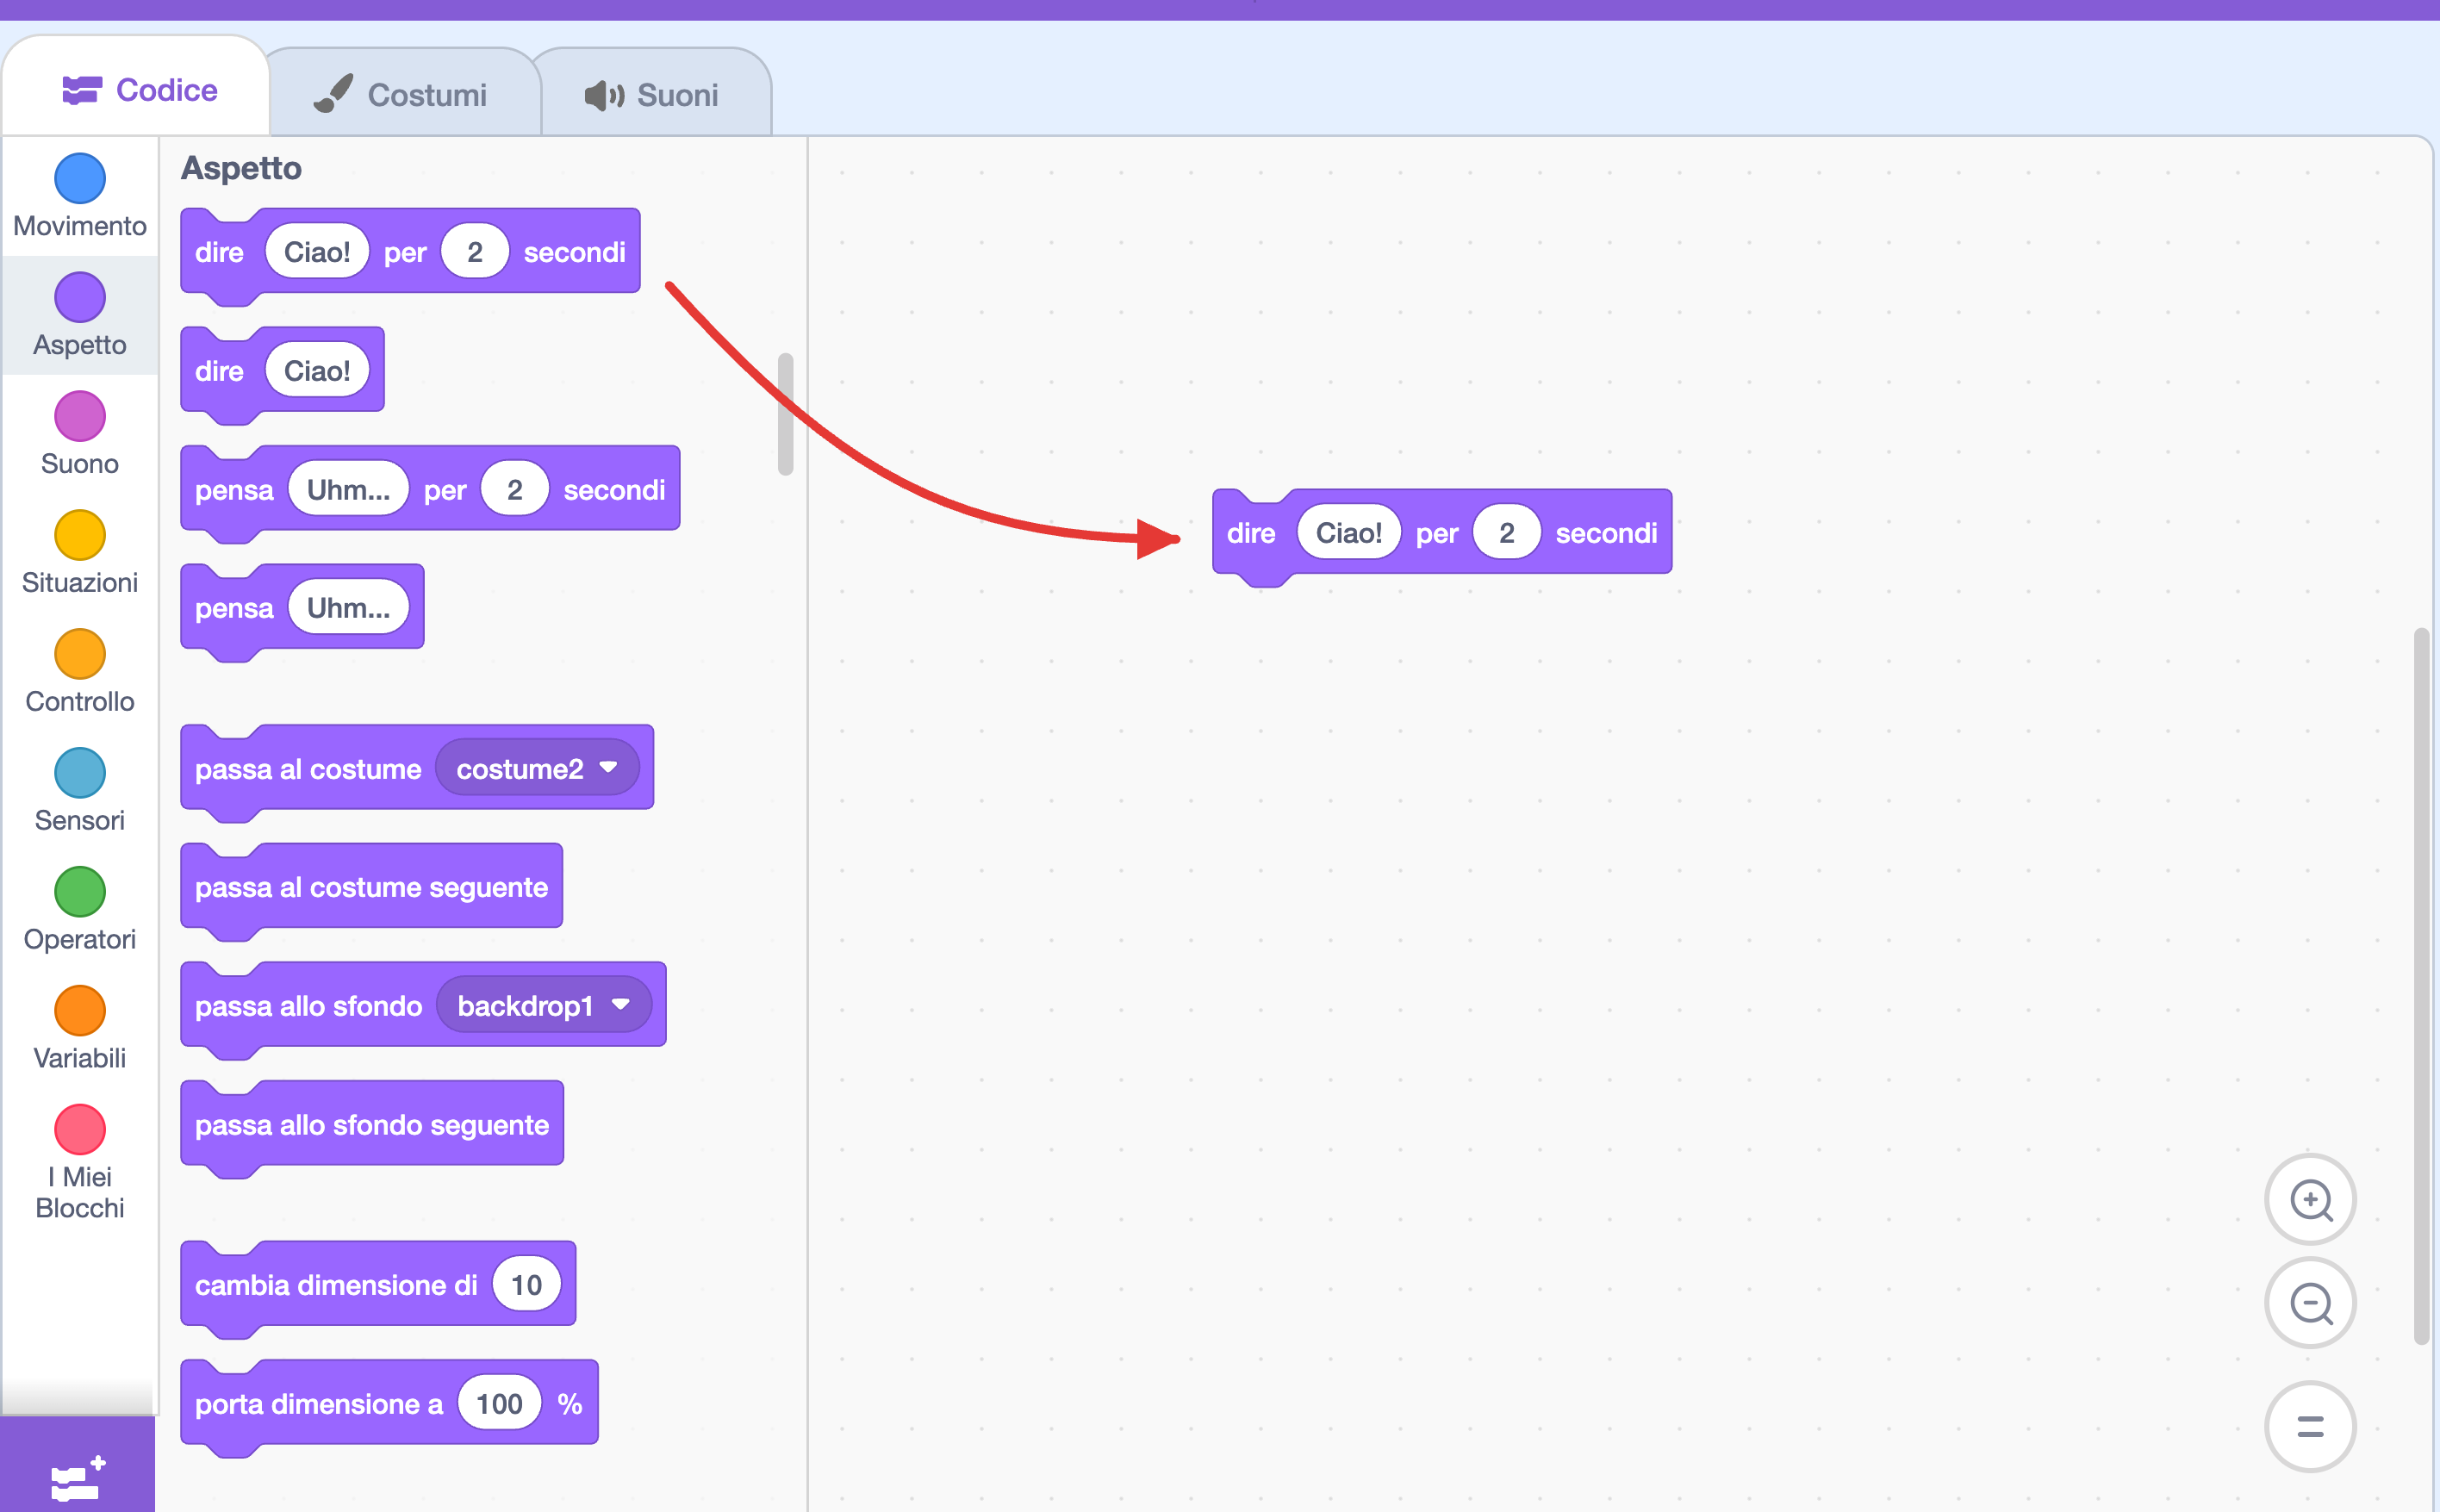
\includegraphics[width=\linewidth]{img/scratch-trascinamento.png}\label{credito:scratch-trascinamento-1}
\end{center}

In questa guida, ci concentreremo su Movimento, Suono, Aspetto, Situazioni e Controllo, mentre Sensori, Operatori e Variabili e liste verranno descritti nel secondo volume.

Dall'Area dei blocchi si possono trascinare i blocchi nell'Area del codice per costruire un programma. I blocchi si agganciano tra loro in sequenza, come pezzi di un puzzle, e ogni sprite esegue le istruzioni dall'alto verso il basso. È possibile spostare, aggiungere o togliere blocchi in qualsiasi momento, modificando così il comportamento dello sprite.

\newpage
Perché Scratch possa eseguire correttamente le istruzioni, i blocchi devono essere incastrati tra loro. Nella figura seguente, il blocco a sinistra è agganciato correttamente, mentre gli altri due non lo sono: se i blocchi restano separati, verranno ignorati da Scratch.

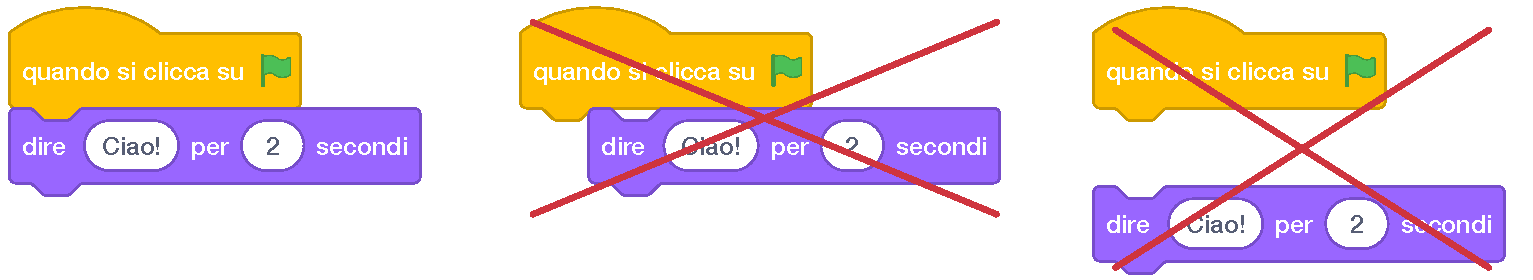
\includegraphics[width=0.9\linewidth]{img/scratchblocks-cap08/pdf/scratch-agganciati.pdf}\label{credito:scratch-agganciati-1}

\Needspace{12\baselineskip}
Il programma, in questo caso, è composto da due istruzioni:

\begin{itemize}
\item
  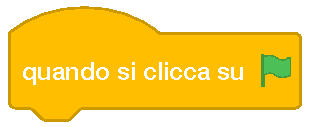
\includegraphics[width=99.5bp]{img/scratchblocks-cap08/pdf/scratch-bandiera.pdf}\label{credito:scratch-bandiera-1} (\textbf{Situazioni}): indica che il programma inizierà quando l'utente cliccherà sul pulsante start (la bandiera verde che si trova sopra allo stage).
\item
  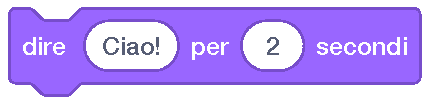
\includegraphics[width=137.5bp]{img/scratchblocks-cap08/pdf/testo-dire-ciao.pdf}\label{credito:testo-dire-ciao-1} (\textbf{Aspetto}): fa comparire sullo sprite un fumetto con la scritta ``Ciao!'' per 2 secondi. Il numero di secondi da inserire dipende dalla lunghezza del testo e dal tempo necessario a chi guarda per leggerlo con calma: per frasi più lunghe può essere utile aumentare l'attesa.
\end{itemize}


In Scratch alcuni blocchi contengono parti già definite e parti ``in bianco'' che possono essere modificate. Queste parti modificabili si chiamano \textbf{parametri}: basta cliccarci sopra per cambiare il valore. Ad esempio, nel blocco 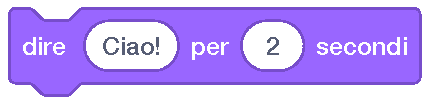
\includegraphics[width=137.5bp]{img/scratchblocks-cap08/pdf/testo-dire-ciao.pdf}\label{credito:testo-dire-ciao-2} è possibile scrivere il testo che comparirà nel fumetto e decidere per quanti secondi mostrarlo.

Fai scegliere a ciascuno un personaggio e due o tre frasi da fargli pronunciare con i blocchi ``dire''.

\newpage
\section{Attività 3: dialogo tra due personaggi}

\ruoliattivita{\ruoloProgrammatore}

\subsection{Sincronizzazione}


Quando ci sono più personaggi, ciascuno può avere il proprio blocco 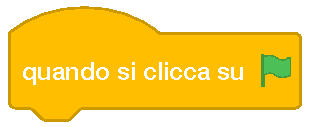
\includegraphics[width=99.5bp]{img/scratchblocks-cap08/pdf/scratch-bandiera.pdf}\label{credito:scratch-bandiera-2}.

In questo caso, tutti gli sprite inizieranno ad eseguire il loro codice nello stesso momento.

Se, ad esempio, abbiamo un blocco 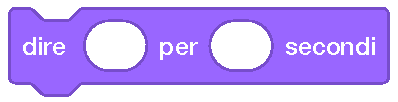
\includegraphics[width=127.5bp]{img/scratchblocks-cap08/pdf/scratch-dire-ciao.pdf}\label{credito:scratch-dire-ciao-1} in ognuno di loro, tutti mostreranno il fumetto contemporaneamente. Se però vogliamo che parlino uno alla volta, o che uno sprite inizi a muoversi solo dopo che un altro ha finito, dobbiamo \textbf{sincronizzare} le loro azioni, cioè decidere l'ordine e i momenti in cui ogni sprite deve attivarsi.

Prendiamo come esempio un dialogo tra un ippopotamo e un ragnetto (mostrato per intero nella figura).

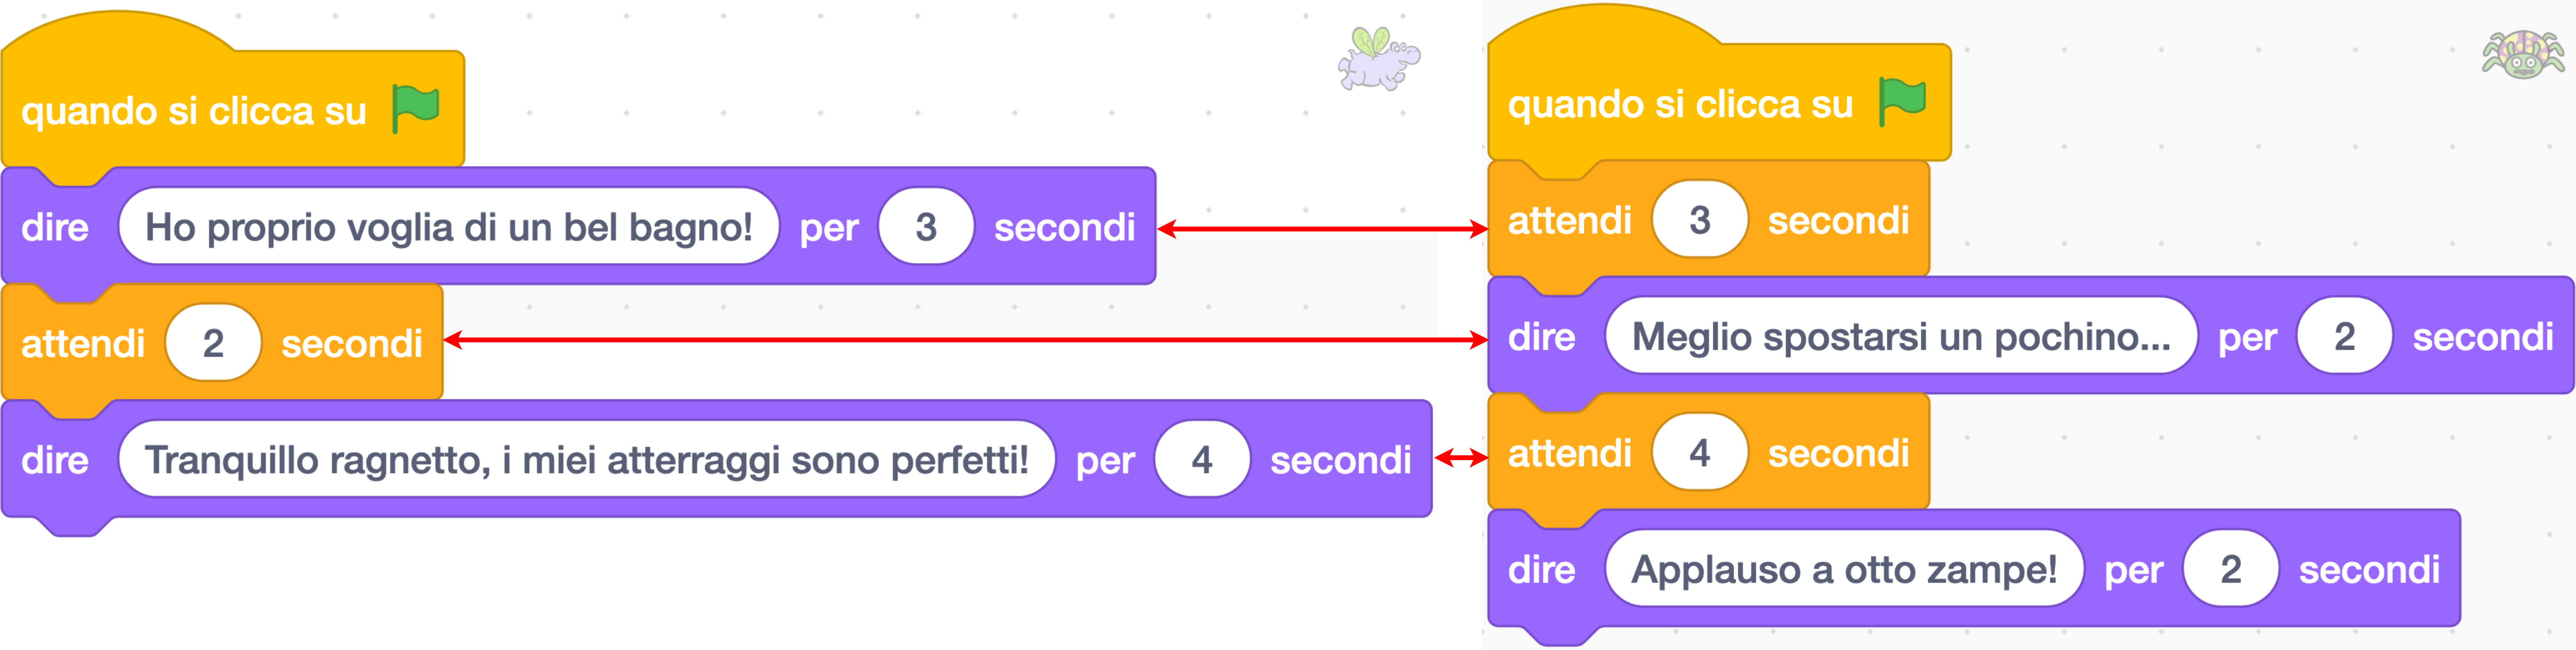
\includegraphics[width=\linewidth]{img/scratch-dialogo.png}\label{credito:scratch-dialogo-1}

L'ippopotamo pronuncia la prima battuta e solo dopo alcuni secondi il ragnetto\footnote{Lo sprite scelto è Ladybug2, che, stando al nome, è una coccinella. Continueremo a chiamarlo ``ragnetto'' per maggiore suggestività. Al lettore pignolo facciamo notare che l'ippopotamo ha due ali da insetto \emoji{wink}} risponde. Per ottenere questo comportamento ordinato non basta mettere i blocchi in sequenza: bisogna dire allo sprite \textbf{quando} deve iniziare la sua azione.


Utilizziamo il blocco 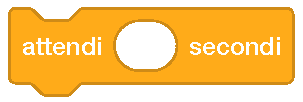
\includegraphics[width=97bp]{img/scratchblocks-cap08/pdf/scratch-attendi.pdf}\label{credito:scratch-attendi-1} (\textbf{Controllo}), qui a fianco, che permette allo sprite di fare una pausa prima di passare alle istruzioni successive. In questo esempio, il ragnetto aspetta 3 secondi, cioè il tempo che serve per far finire la frase all'ippopotamo: come si vede nella figura, i blocchi attendi permettono ai personaggi di parlare uno dopo l'altro, senza sovrapporsi.


Prima di programmare può essere utile creare un piccolo storyboard: una sequenza di vignette o appunti che raccontano, passo dopo passo, cosa succederà nella storia o nell'animazione. Questo passaggio permette a ciascuno di pianificare con chiarezza le scene, decidere chi parla, chi si muove e quando, e trasformare l'idea in un progetto ordinato. Lavorare con uno storyboard evita confusione in fase di programmazione e aiuta a mantenere una visione d'insieme del progetto.

\begin{center}
\setlength{\tabcolsep}{4pt}
\setlength{\arrayrulewidth}{0.5pt}
\renewcommand{\arraystretch}{1.45}
\begin{tabular}{|*{2}{>{\centering\arraybackslash}m{\dimexpr0.4\linewidth-2\tabcolsep-1.25\arrayrulewidth\relax}|>{\centering\arraybackslash}m{\dimexpr0.1\linewidth-2\tabcolsep-1.25\arrayrulewidth\relax}|}}
\arrayrulecolor{black!40}
\hline
\rowcolor{black!12}
\multicolumn{2}{|>{\centering\arraybackslash}m{\dimexpr0.5\linewidth-2\tabcolsep-1.5\arrayrulewidth\relax}|}{\textbf{Personaggio: Lupo}} &
\multicolumn{2}{>{\centering\arraybackslash}m{\dimexpr0.5\linewidth-2\tabcolsep-1.5\arrayrulewidth\relax}|}{\textbf{Personaggio: Cappuccetto Rosso}} \\
\hline
Ciao bella bambina! & 3 & \multirow[t]{2}{*}{ATTENDI} & \multirow[t]{2}{*}{5} \\
\cline{1-2}
Come ti chiami? & 2 & & \\
\hline
ATTENDI & 4 & Mi chiamo Cappuccetto Rosso! & 4 \\
\hline
Ma che bel nome! & 2 & ATTENDI & 2 \\
\hline
\end{tabular}
\end{center}



\subsection{Ripetizione}\label{ripetizione}

\noindent
\begin{minipage}[t]{0.28\linewidth}
\vspace{0pt}
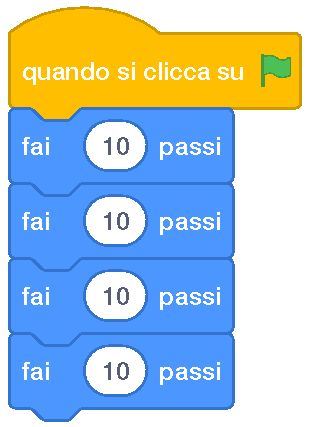
\includegraphics[width=99.5bp]{img/scratchblocks-cap08/pdf/scratch-programma-lungo.pdf}\label{credito:scratch-programma-lungo-1}
\end{minipage}\hfill
\begin{minipage}[t]{0.68\linewidth}
\vspace{0pt}
Supponiamo che il ragnetto non si fidi delle doti dell'ippopotamo e voglia spostarsi sullo schermo. Per farlo potrebbe usare più volte il blocco 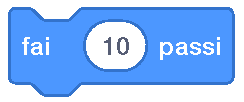
\includegraphics[width=78bp]{img/scratchblocks-cap08/pdf/scratch-fai10.pdf}\label{credito:scratch-fai10-1}, come nel programma qui a fianco, ma il programma diventerebbe lungo, difficile da leggere e da modificare.
\end{minipage}

\noindent
\begin{minipage}[t]{0.28\linewidth}
\vspace{0pt}
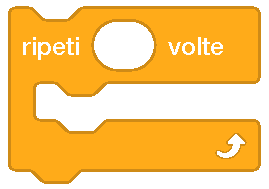
\includegraphics[width=86bp]{img/scratchblocks-cap08/pdf/scratch-ripeti-vuoto.pdf}\label{credito:scratch-ripeti-vuoto-1}
\end{minipage}\hfill
\begin{minipage}[t]{0.68\linewidth}
\vspace{0pt}
Per rendere il codice più semplice possiamo usare il blocco \textbf{ripeti \ldots{} volte} (\textbf{Controllo}). Questo blocco ha la forma di una ``C'' aperta: la sequenza delle istruzioni inserite al suo interno verrà ripetuta per il numero di volte indicato. Le istruzioni che si trovano fuori dalla ``C'' non verranno ripetute.
\end{minipage}

\Needspace{14\baselineskip}
\begin{consiglio}[Maestr* si è buggato... non ripete niente!]

È utile far notare che, soprattutto all'inizio, alunni e alunne incastrano i blocchi nel punto sbagliato: ad esempio, può capitare che il blocco 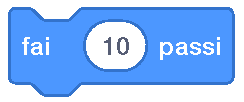
\includegraphics[width=78bp]{img/scratchblocks-cap08/pdf/scratch-fai10.pdf}\label{credito:scratch-fai10-2} venga messo prima o dopo la ``C'', pensando che venga comunque ripetuto (nella figura seguente, solo il programma a sinistra ripete il movimento). Mostrare loro l'effetto dell'errore aiuta a comprendere meglio la logica della ripetizione e l'importanza della posizione dei blocchi.

\begin{center}
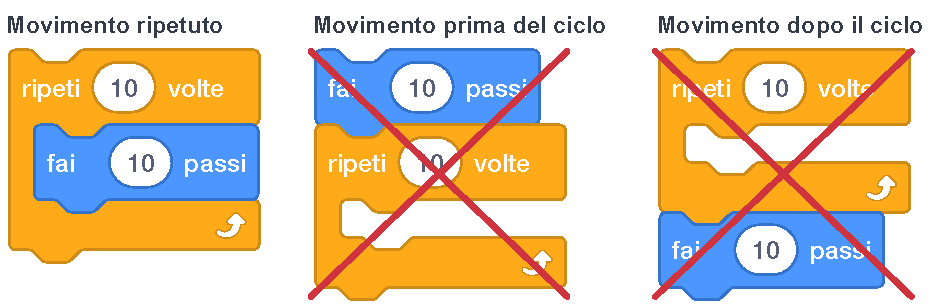
\includegraphics[width=0.92\linewidth]{img/scratchblocks-cap08/pdf/scratch-ripeti-completo.pdf}\label{credito:scratch-ripeti-completo-1}
\end{center}

\end{consiglio}
\newpage
\subsection{Ripetizione infinita}\label{ripetizione-infinita}

Possiamo anche ripetere una sequenza di blocchi all'infinito con il blocco \textbf{per sempre} (\textbf{Controllo}).

\begin{center}
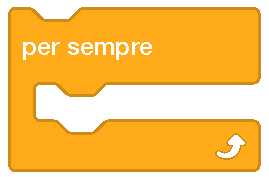
\includegraphics[width=86bp]{img/scratchblocks-cap08/pdf/scratch-persempre-vuoto.pdf}\label{credito:scratch-persempre-vuoto-1}
\end{center}

A differenza del blocco \textbf{ripeti \ldots{} volte}, questo blocco non ha l'incastro sul fondo: significa che il programma continuerà a eseguire all'infinito le istruzioni contenute al suo interno, senza arrivare mai a un blocco successivo. Come nel caso di \textbf{ripeti \ldots{} volte}, verranno ripetuti solo i blocchi inseriti dentro la ``C''.

\noindent
\begin{minipage}[t]{0.34\linewidth}
\vspace{0pt}
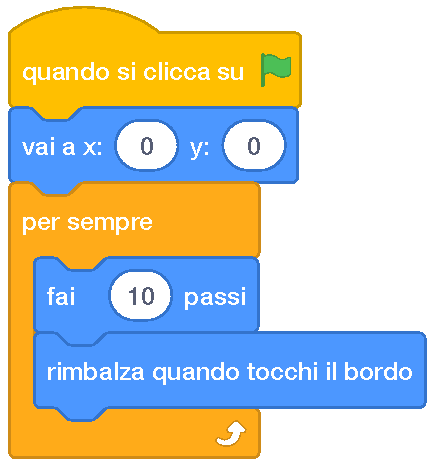
\includegraphics[width=139bp]{img/scratchblocks-cap08/pdf/scratch-persempre1.pdf}\label{credito:scratch-persempre1-1}
\end{minipage}\hfill
\begin{minipage}[t]{0.62\linewidth}
\vspace{0pt}
Nel codice qui a fianco, lo sprite viene prima posizionato al centro dello stage (x: 0, y: 0) e poi, \textbf{per sempre}, fa 10 passi e rimbalza quando tocca il bordo: si muoverà quindi in continuazione avanti e indietro.
\end{minipage}


\Needspace{0.35\textheight}
\begin{consiglio}[Maestr* si è buggato... non si muove!]

\ruoliattivita{\ruoloEsecutore}

\noindent
\begin{minipage}[t]{0.34\linewidth}
\vspace{0pt}
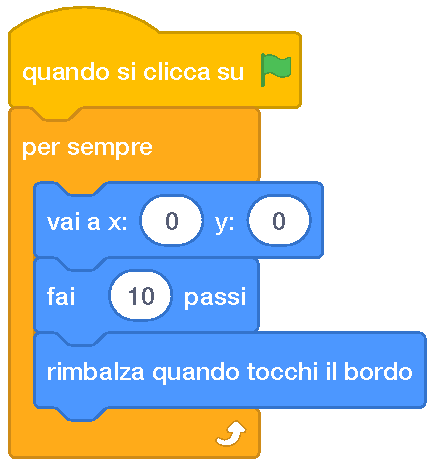
\includegraphics[width=\linewidth]{img/scratchblocks-cap08/pdf/scratch-persempre2.pdf}\label{credito:scratch-persempre2-1}
\end{minipage}\hfill
\begin{minipage}[t]{0.62\linewidth}
\vspace{0pt}
Nel codice qui a fianco, invece, anche il blocco 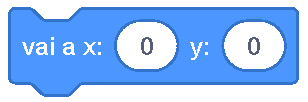
\includegraphics[width=98.5bp]{img/scratchblocks-cap08/pdf/scratch-vai-centro.pdf}\label{credito:scratch-vai-centro-1} è inserito dentro la ``C'': in questo caso lo sprite torna al centro dello stage ad ogni ripetizione, fa solo pochi passi e poi ricomincia subito da capo. Il movimento è impercettibile e può sembrare che lo sprite ``non si muova''. In questi casi, può essere utile chiedere al proprio alunno/a di leggere il codice ad alta voce, passo per passo (``cosa succede per primo? e poi? e poi?'') per facilitare il ragionamento di studenti e studentesse sul comportamento dei propri blocchi.
\end{minipage}

\end{consiglio}

\clearpage
\section{Attività 4: movimenti precisi}

\ruoliattivita{\ruoloProgrammatore}

Ogni sprite, oltre al nome, ha diverse proprietà visibili nell'Area degli sprite. In questa sezione è possibile vedere e modificare informazioni come posizione, direzione, dimensione e visibilità, come mostrato nell'immagine.


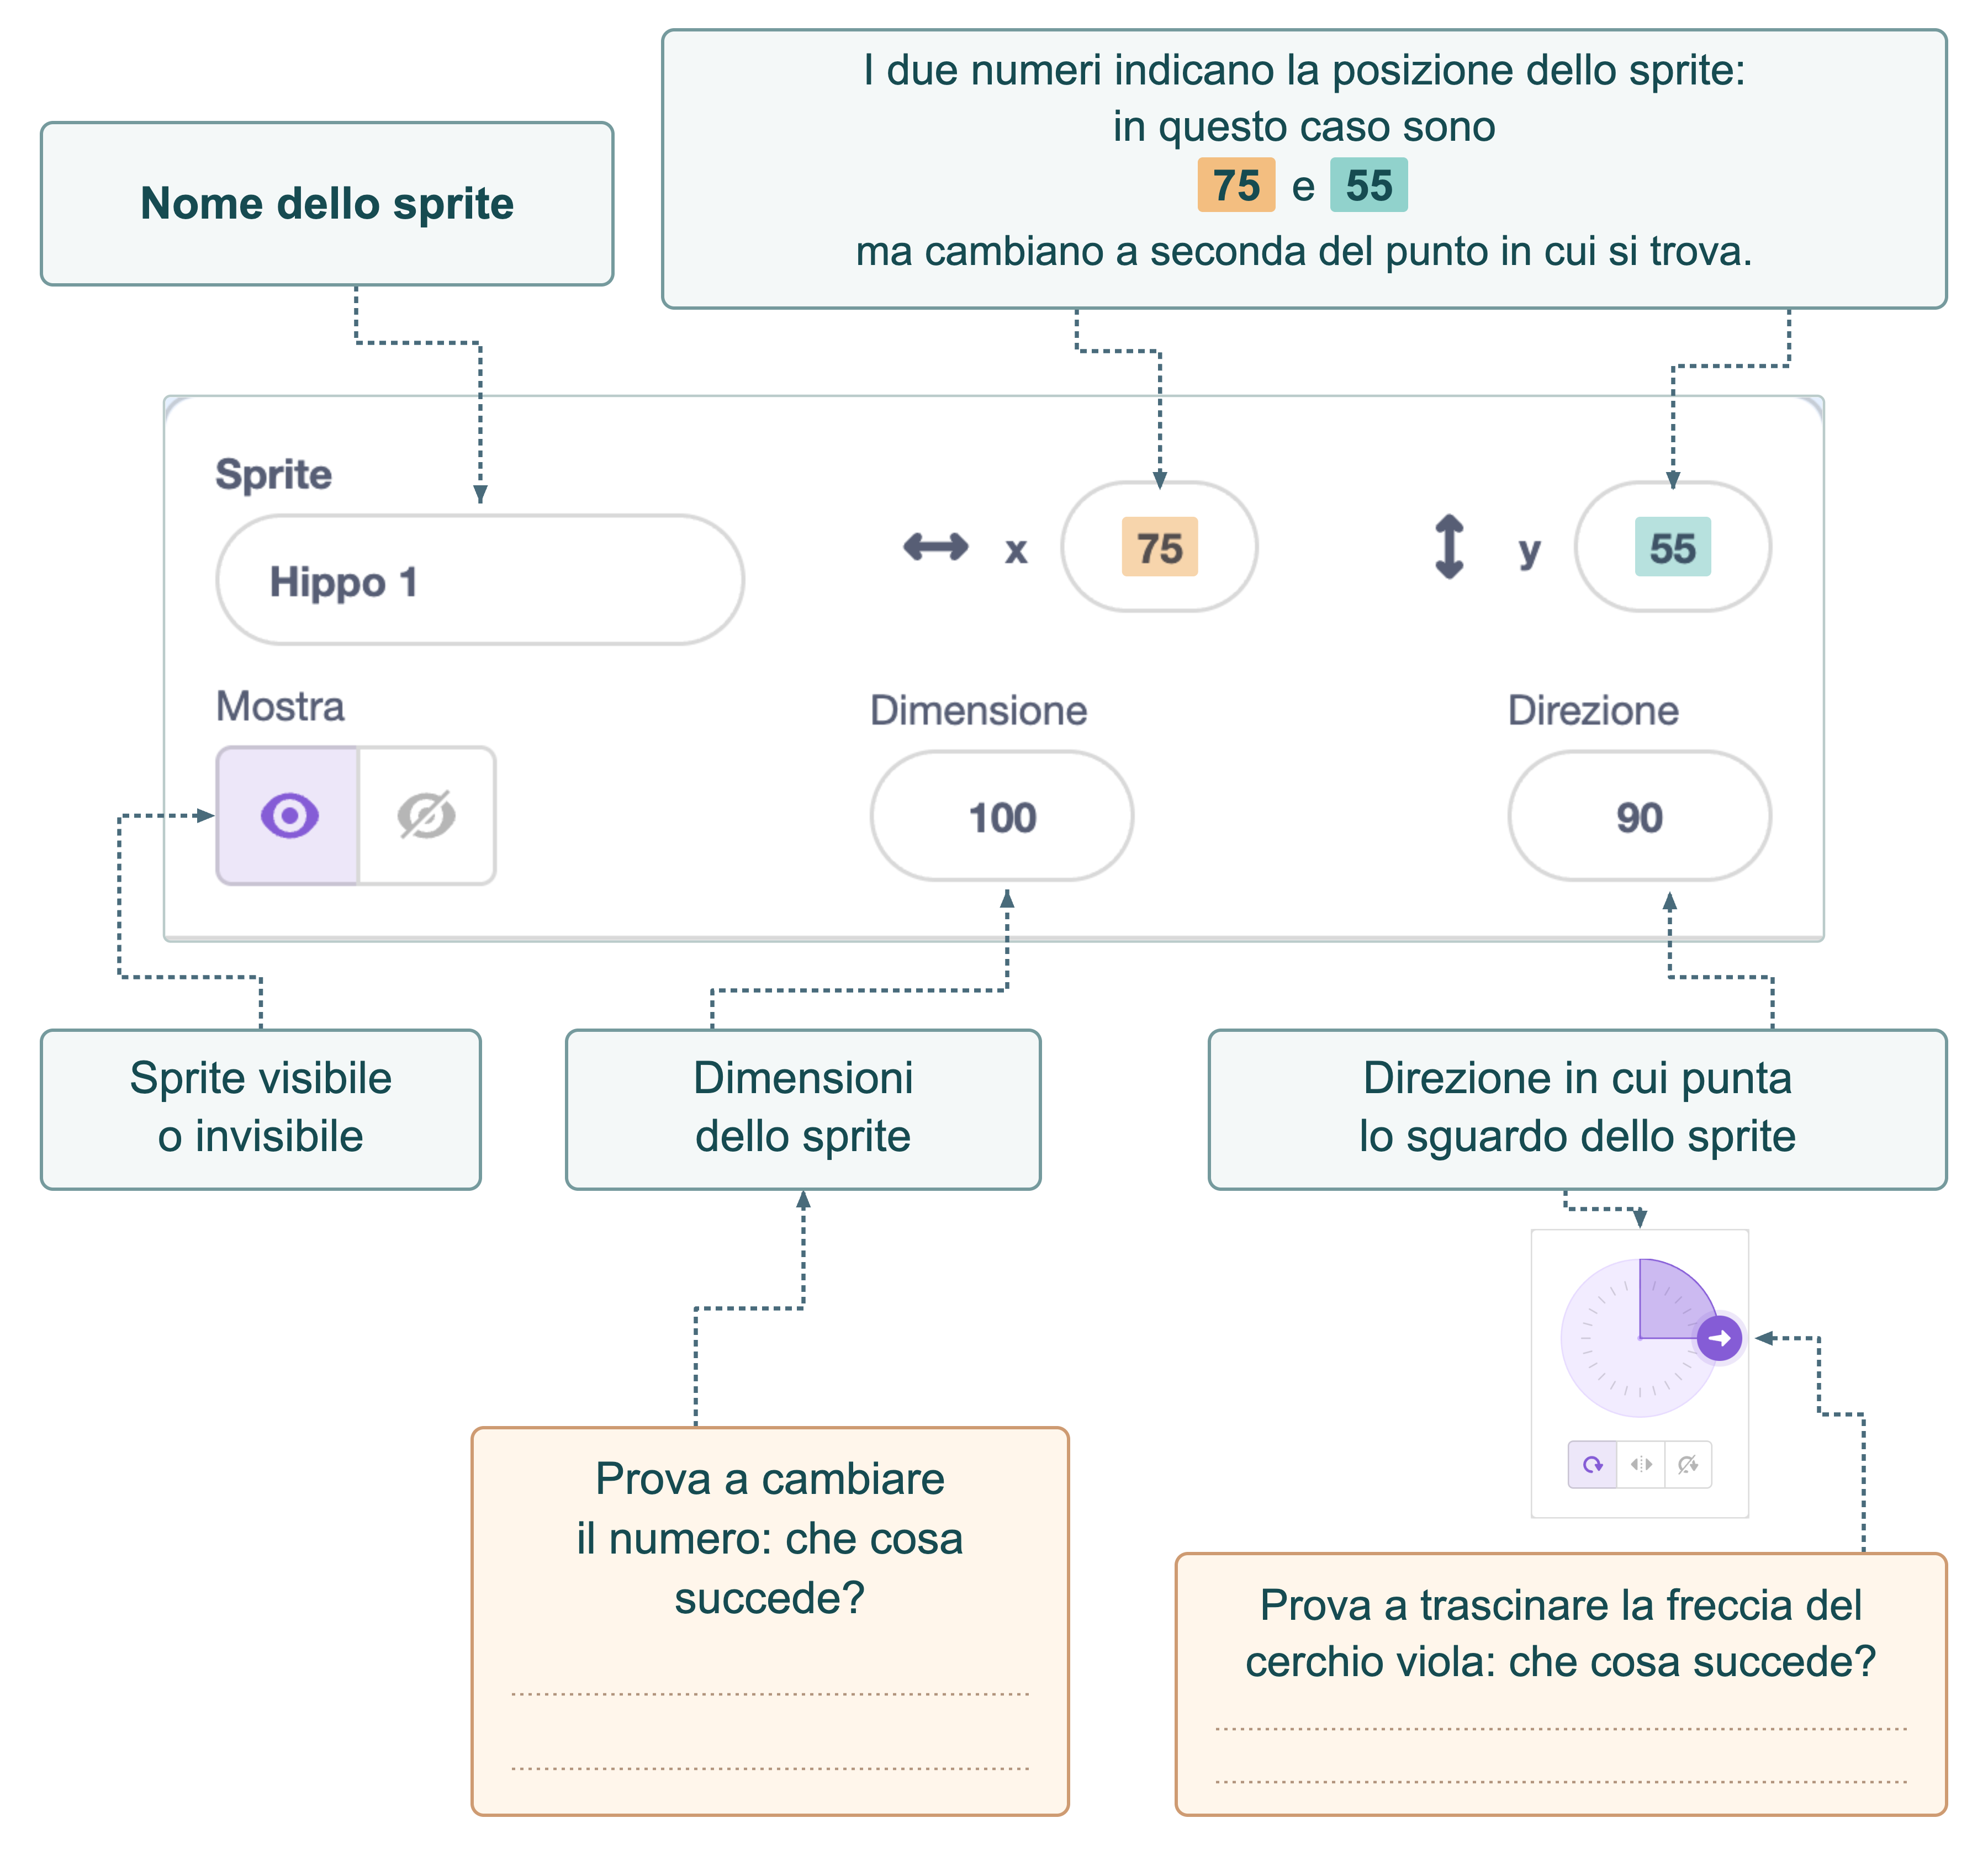
\includegraphics[width=0.9\linewidth]{img/scratch-proprieta-sprite.png}\label{credito:scratch-proprieta-sprite-1}



Incoraggiate alunni e alunne ad esplorare cosa succede cambiando la proprietà \textbf{dimensione} e la proprietà \textbf{direzione} nell'Area degli sprite.


\subsection{La posizione}\label{la-posizione}

\noindent
\begin{minipage}[t]{0.49\linewidth}
\vspace{0pt}
Lo sfondo visibile nell'immagine è uno degli sfondi predefiniti di Scratch (\textbf{Xy-grid}). Mostra allo stesso tempo lo stage e il sistema di coordinate cartesiane che lo struttura. La larghezza misura 480 unità (240 a destra e 240 a sinistra del centro) e l'altezza 360 unità (180 sopra e 180 sotto il centro). Il punto centrale dello stage è indicato dalle coordinate x=0 e y=0: la linea arancione (orizzontale) rappresenta l'asse X, la linea blu (verticale) l'asse Y.
\end{minipage}\hfill
\begin{minipage}[t]{0.48\linewidth}
\vspace{0pt}
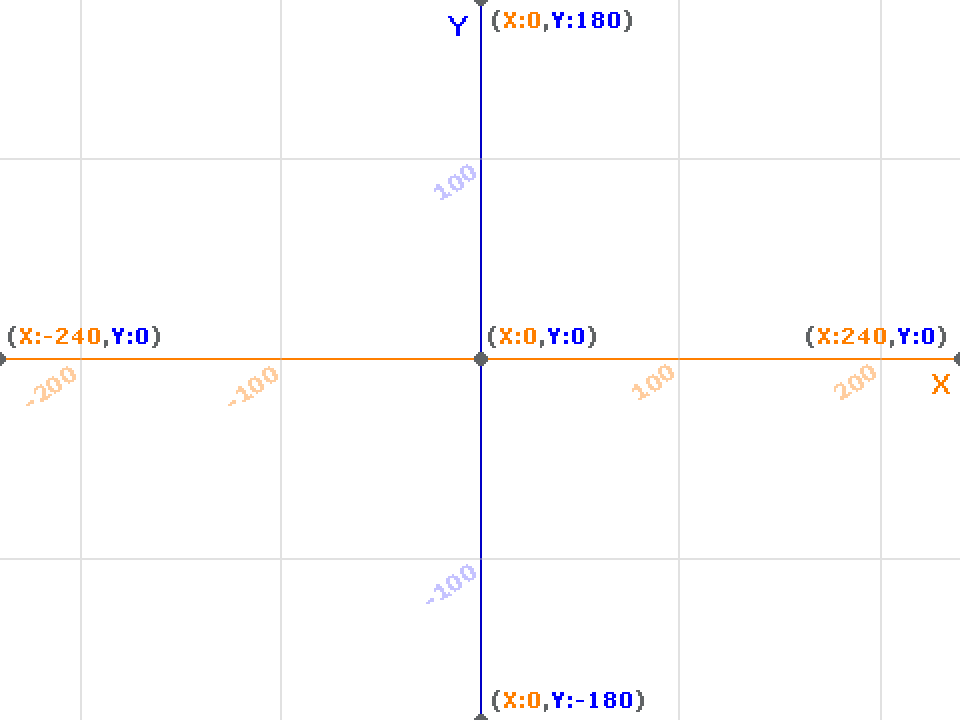
\includegraphics[width=\linewidth]{img/scratch-xy-grid.png}\label{credito:scratch-xy-grid-1}
\end{minipage}
\par

Sebbene in terza primaria sia possibile che piano cartesiano e numeri negativi non siano ancora stati oggetto di insegnamento esplicito, Scratch offre la possibilità di incontrarli in modo naturale e graduale: il semplice fatto di copiare i valori indicati, provare a modificarli e osservare cosa succede ai personaggi può aiutare a orientarsi sullo stage e a prendere confidenza con l'idea di movimento sul piano.

Per questa esplorazione, chiedete di selezionare lo sfondo \textbf{Xy-grid} e lo sprite \textbf{Ball} dalla libreria di Scratch.  Incoraggiate alunni e alunne a esplorare cosa accade cambiando la posizione dello sprite: prima spostandolo con il mouse e osservando come cambiano i valori di x e y, poi scrivendo direttamente dei valori nelle caselle x e y dell'Area degli sprite e osservando dove ``salta'' il personaggio.


\begin{minipage}{\linewidth}
\centering
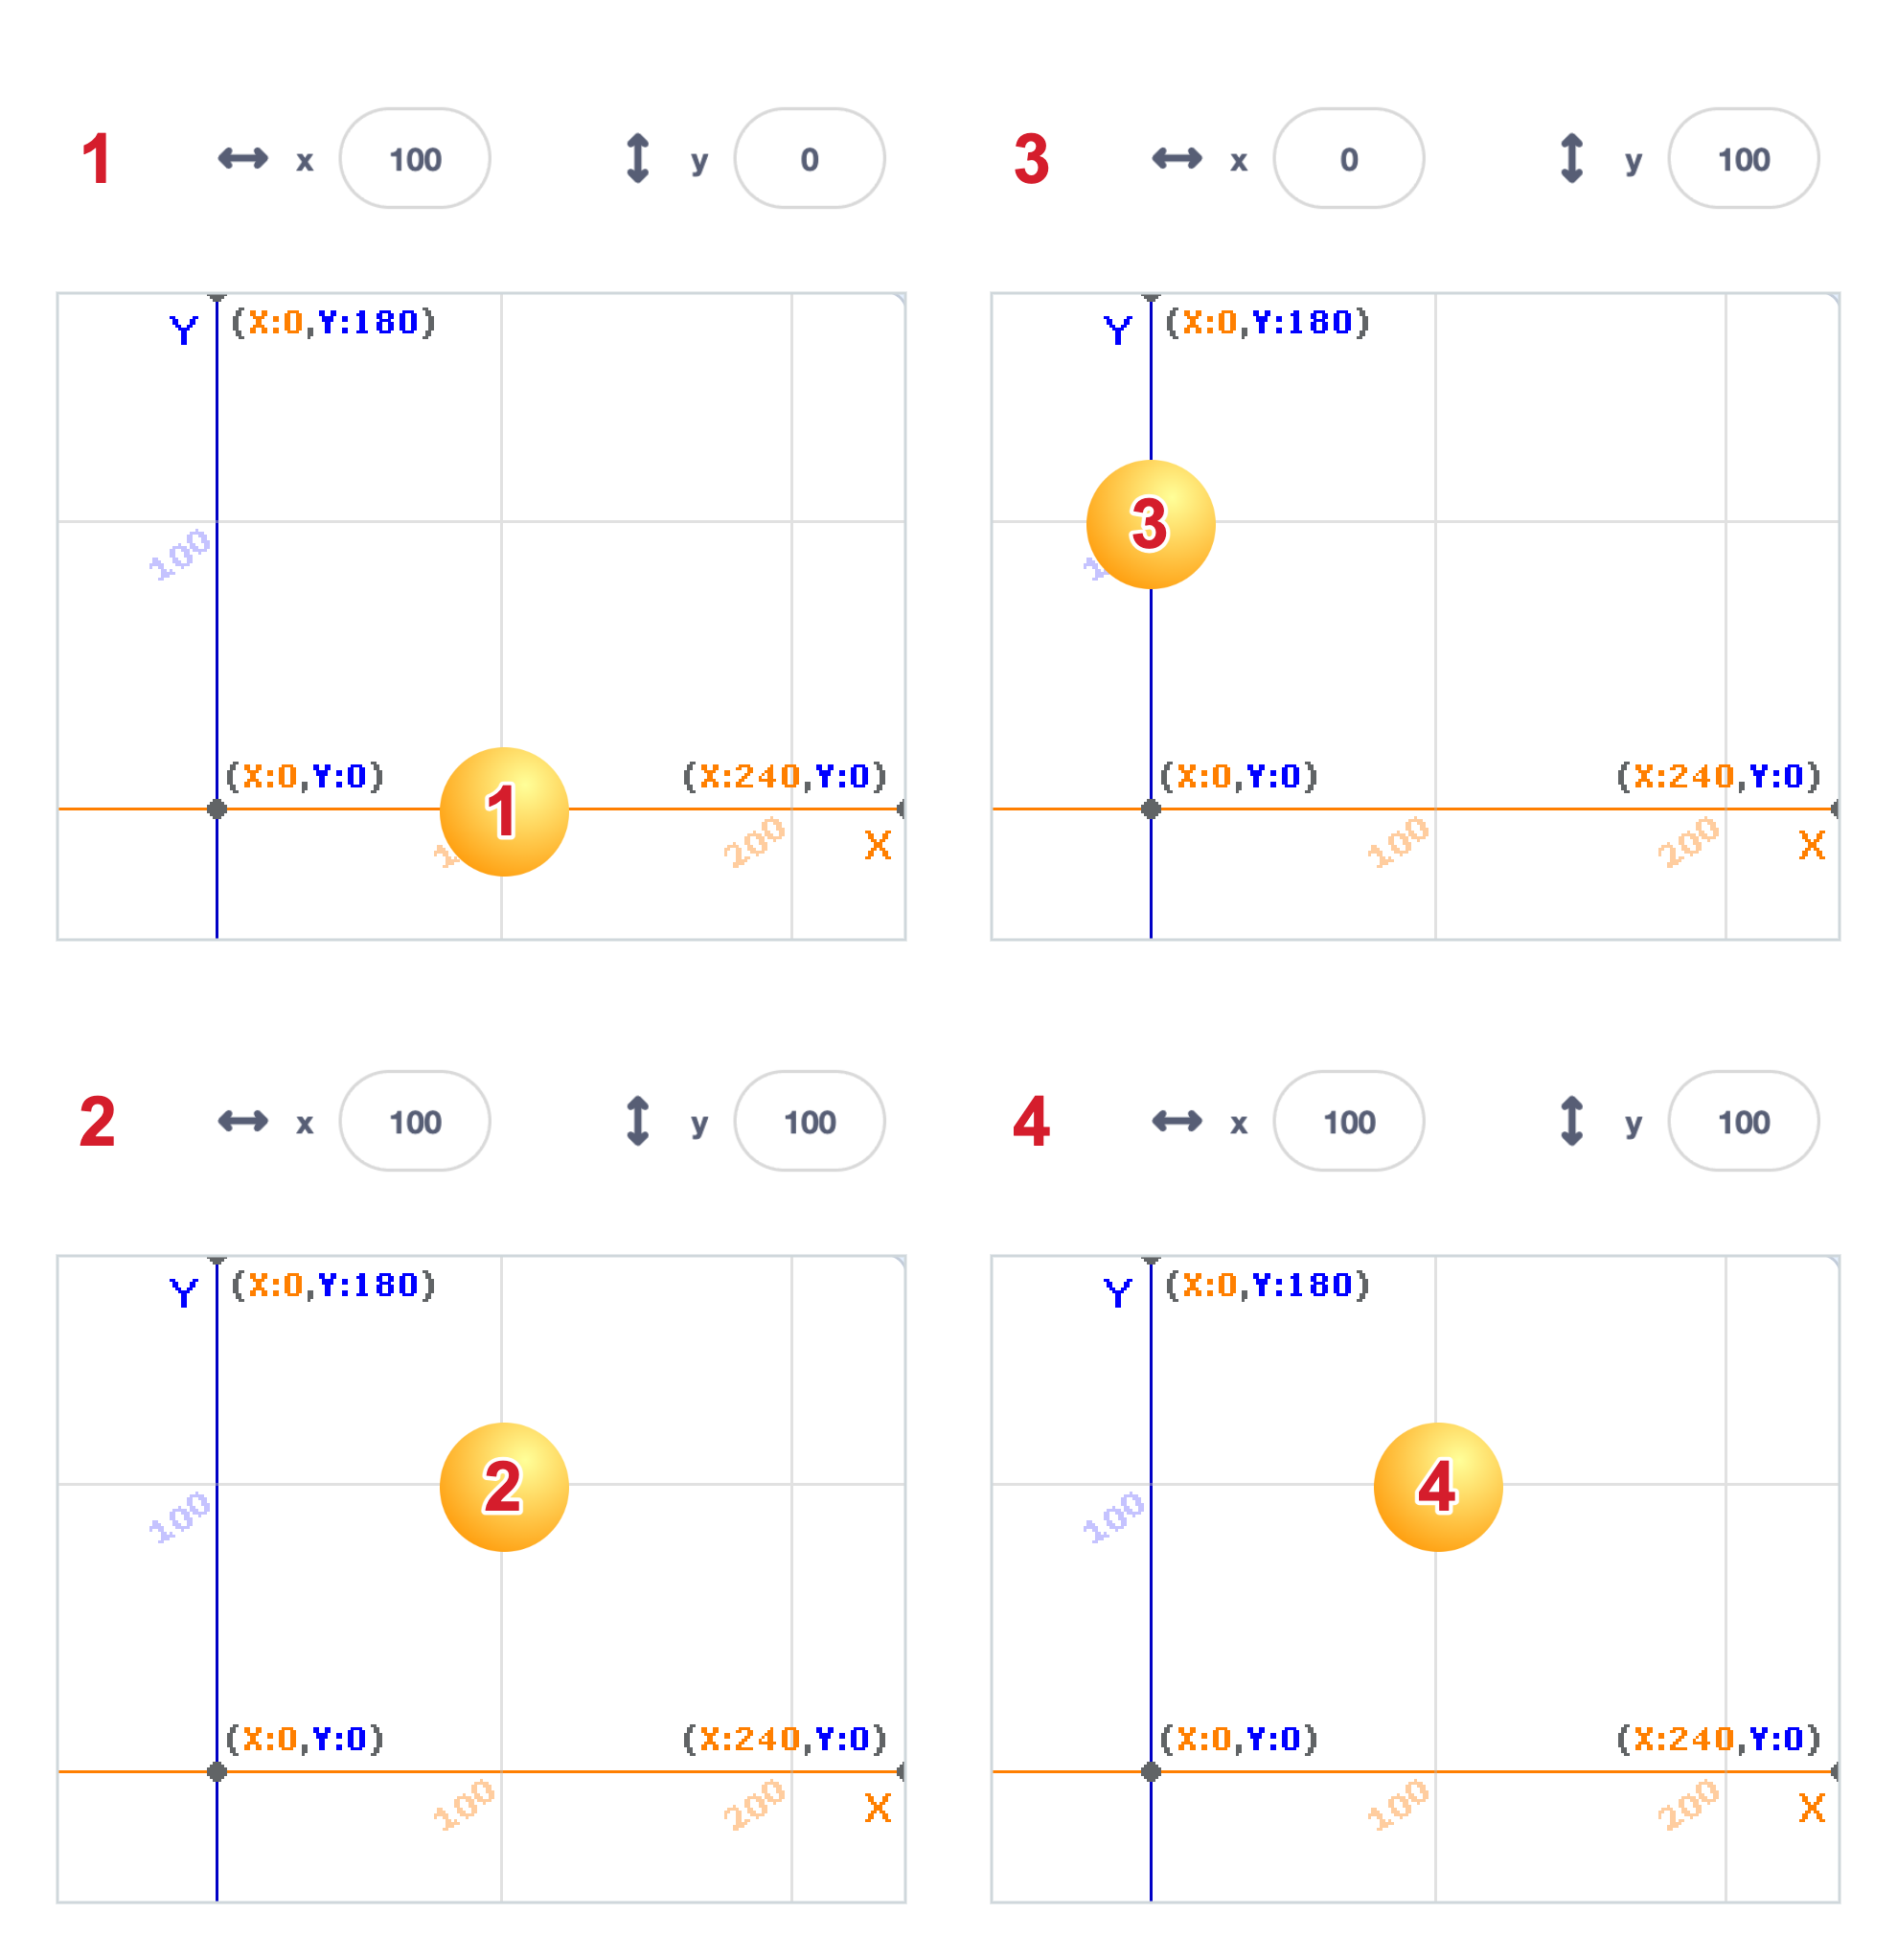
\includegraphics[width=0.8\linewidth]{img/scratch-coordinate.png}\label{credito:scratch-coordinate-1}
\end{minipage}

\section{Attività 5: posizionare un personaggio}

\ruoliattivita{\ruoloProgrammatore}

\subsection{Scegliere una posizione}\label{scegliere-una-posizione}

Il blocco 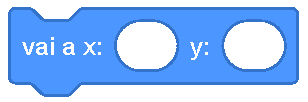
\includegraphics[width=98.5bp]{img/scratchblocks-cap08/pdf/scratch-vai-a.pdf}\label{credito:scratch-vai-a-1} (\textbf{Movimento}) permette di posizionare lo sprite in una precisa posizione dello stage. Per trovare le coordinate da inserire, bisogna (1) spostare lo sprite con il mouse nella posizione desiderata, (2) leggere i valori \emph{x} e \emph{y} riportati nell'Area degli sprite e (3) copiarli dentro il blocco. In questo modo il personaggio si sposterà sempre nel punto scelto. Questa procedura aiuta alunni e alunne a scoprire che lo sprite può essere posizionato sia ``a mano'' nell'interfaccia, come se fosse telecomandato, sia usando il blocco di movimento, cioè \textbf{pianificando} in anticipo le azioni. Questo passaggio può aiutare a capire la differenza tra muovere direttamente il personaggio e farlo muovere da solo seguendo le istruzioni del programma.

Proponete di copiare un programma che usa il blocco \textbf{vai a} per fissare la posizione di partenza, ad esempio:
\begin{center}
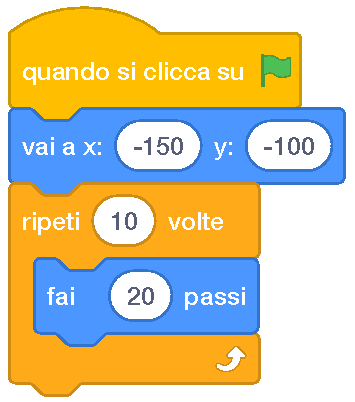
\includegraphics[width=113.5bp]{img/scratchblocks-cap08/pdf/testo-posizione-iniziale.pdf}\label{credito:testo-posizione-iniziale-1}
\end{center}
Incoraggiate bambini e bambine a provare a far partire il personaggio in diversi punti dello schermo, modificando le coordinate di partenza.

\begin{consiglio}[Maestr* si è buggato... perché non comincia come voglio io?]

Al termine dell'esecuzione del programma, può capitare che il personaggio resti in una posizione sullo stage non desiderata. Quando si clicca di nuovo sulla bandierina verde, lo sprite ricomincia a muoversi proprio da lì, rovinando l'effetto voluto.

Questo accade perché ogni personaggio possiede un proprio \textbf{stato}, cioè un insieme di informazioni che Scratch conserva: posizione, direzione, dimensione, visibilità, e così via. In pratica, lo sprite non ``si resetta da solo'': si comporta come un attore un po' distratto, che riparte da dove era rimasto se non gli viene detto con precisione cosa fare.

Per questo è importante inserire all'inizio dello script i blocchi che fissano la posizione di partenza (e, se serve, dimensione e direzione). Un buon trucco in classe è chiedere a ciascuno di leggere a voce alta il proprio codice passo per passo chiedendosi: ``Dove sta il personaggio adesso? Dove gli ho detto di andare? Da dove sta ripartendo?''

Questo aiuta a capire che anche la posizione iniziale fa parte della programmazione.

\end{consiglio}


\subsection{Scegliere una direzione}\label{scegliere-una-direzione}

Nell'Attività precedente abbiamo chiesto agli alunni e alle alunne di esplorare il concetto di direzione. La direzione indica ``dove lo sprite sta guardando'': è come girarsi prima di iniziare a camminare. Come per la posizione, oltre a scegliere la direzione tramite l'interfaccia, è possibile utilizzare il blocco 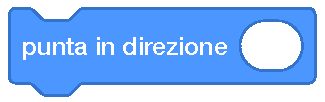
\includegraphics[width=104bp]{img/scratchblocks-cap08/pdf/scratch-punta-direzione.pdf}\label{credito:scratch-punta-direzione-1} (\textbf{Movimento}) per pianificare la direzione del movimento.

Questo blocco funziona con gli angoli misurati in gradi e il valore fa riferimento all'ampiezza dell'angolo centrato nell'origine del sistema di riferimento che struttura lo stage e che ha: un lato sul semiasse Y positivo e il secondo lato dato dalla direzione in cui punta lo ``sguardo dello sprite''. Ad esempio, il valore 0 in questo blocco indica che lo sprite deve puntare lo sguardo in una direzione che formi un angolo di ampiezza 0° con il semiasse positivo Y: quindi, lo sprite punterà lo sguardo verso l'alto; inserendo il valore 180 punterà lo sguardo verso il basso, inserendo -90 punterà lo sguardo verso sinistra e con 90 verso destra, come mostrato nella figura~\ref{fig:direzioni-assolute}.

\begin{figure}
  \begin{center}
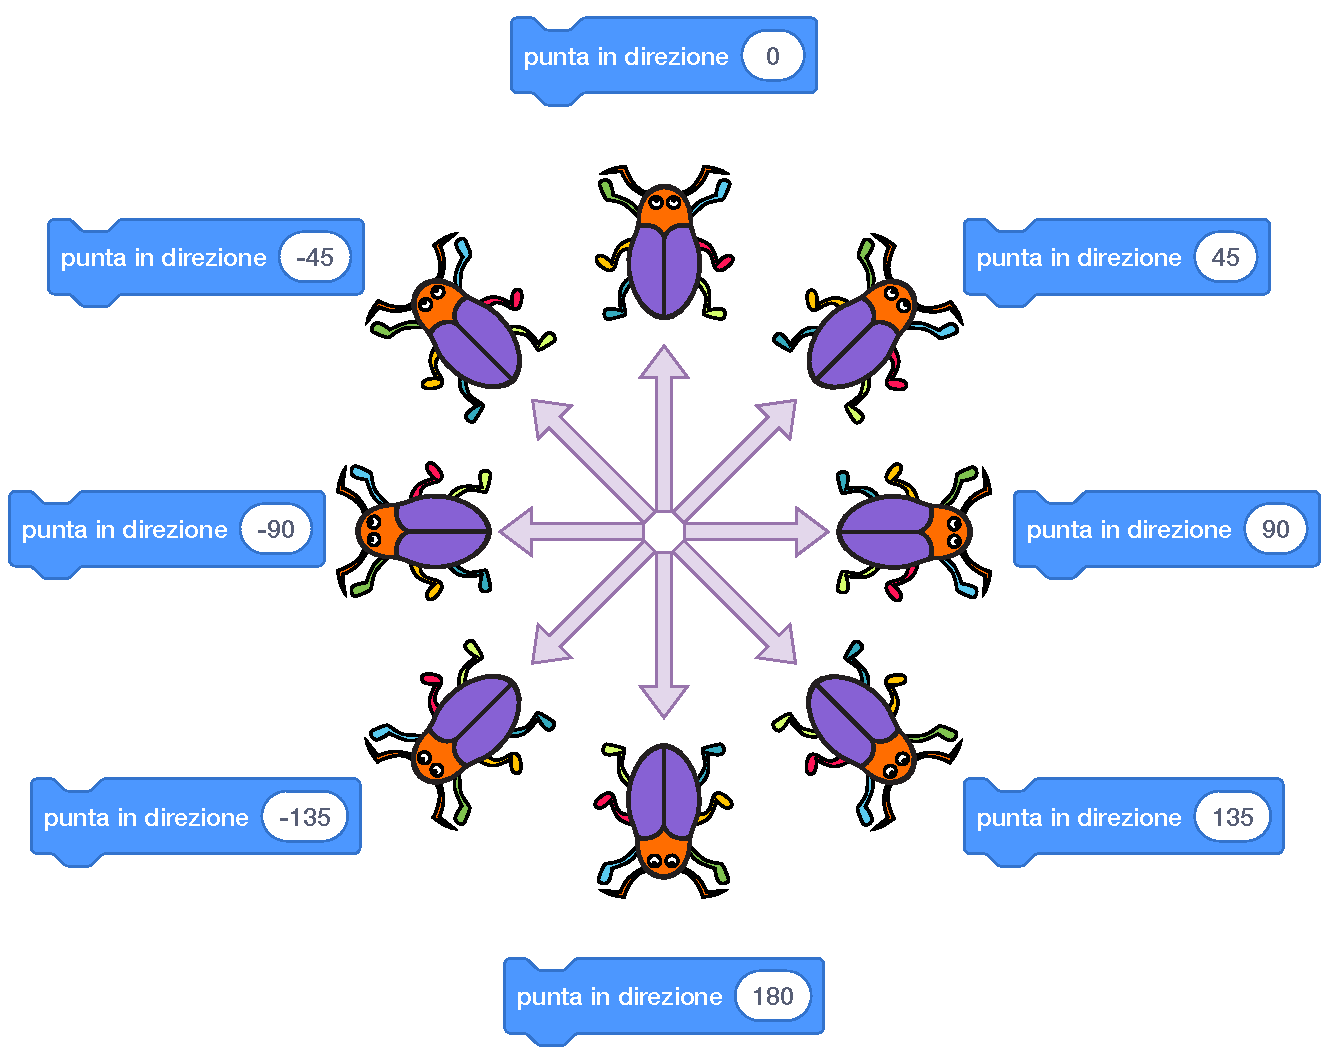
\includegraphics[width=\linewidth]{img/scratchblocks-cap08/pdf/figure-rosa-venti.pdf}\label{credito:figure-rosa-venti-1}
  \end{center}
  \caption{Effetti del blocco \textbf{punta in direzione...}}
  \label{fig:direzioni-assolute}
\end{figure}



Esiste anche un secondo modo per cambiare direzione: la \textbf{rotazione relativa}. È simile ai comandi ``gira a sinistra'' e ``gira a destra'' visti nel Capitolo~\ref{capitolo-7-code.org} su Code.org, ma in Scratch si realizza tramite i blocchi 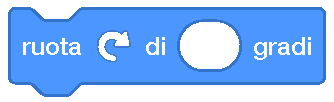
\includegraphics[width=107bp]{img/scratchblocks-cap08/pdf/scratch-ruota-orario.pdf}\label{credito:scratch-ruota-orario-1} (\textbf{Movimento}), in senso orario o antiorario, indicato dalla freccia sul blocco (vedi Figura~\ref{fig:direzioni-relative}).

Questi blocchi fanno ruotare lo sprite attorno al proprio centro e di un angolo dell'ampiezza in gradi indicata rispetto alla direzione in cui sta guardando in quel momento, e non verso una direzione assoluta. Richiedono familiarità con il concetto di angolo, che in terza primaria potrebbe non essere ancora stato affrontato formalmente, ma questi blocchi possono essere utili per comprendere meglio come funziona il movimento e per rispondere agli errori più comuni degli alunni.

\begin{figure}[!htb]
  \centering
  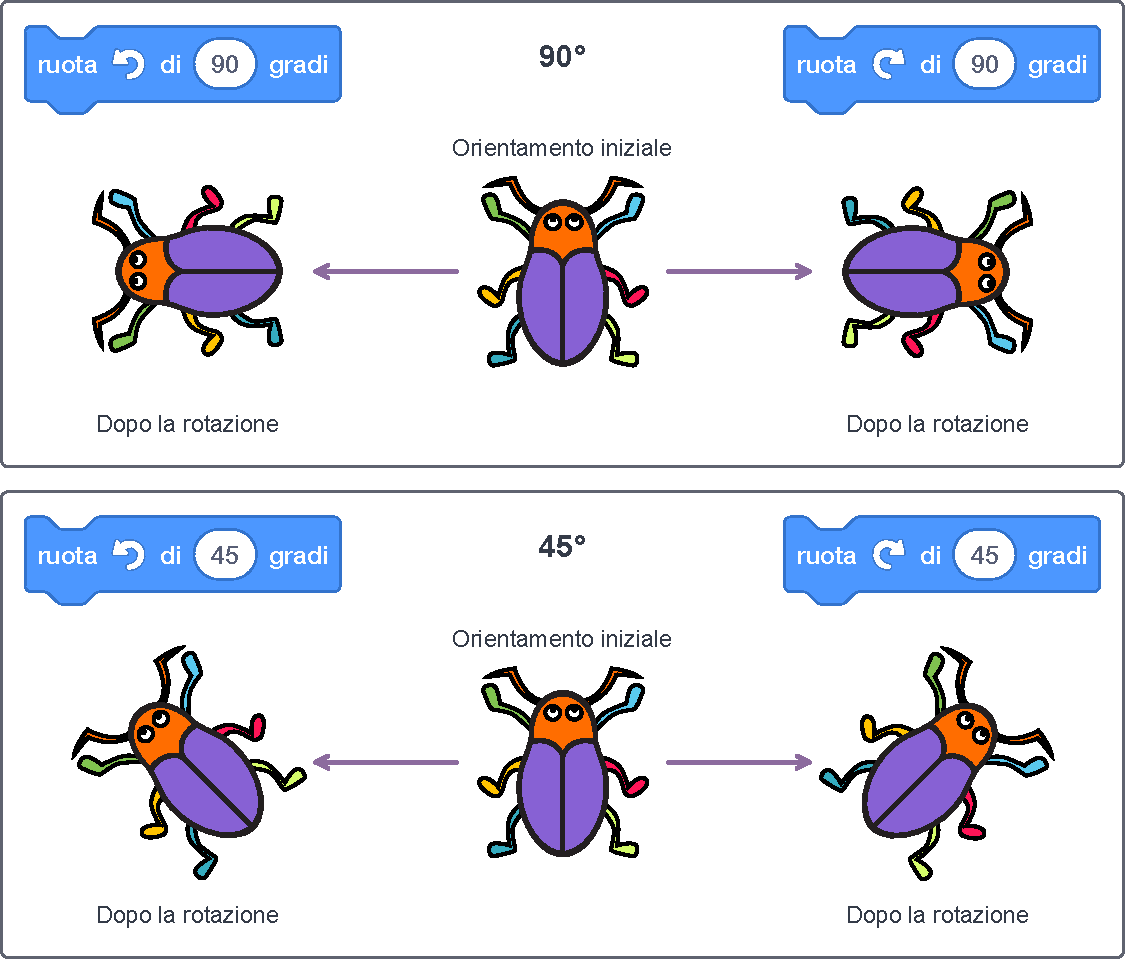
\includegraphics[width=\linewidth]{img/scratchblocks-cap08/pdf/figure-angoli.pdf}
  \label{credito:figure-angoli-1}
  \caption{Effetti del blocco \textbf{ruota...}}
  \label{fig:direzioni-relative}
\end{figure}

\subsection{Approfondimento: spostamenti}\label{approfondimento-spostamenti-assoluti-e-relativi}

I comandi di movimento disponibili in Scratch sono molti di più di quelli proposti nelle attività viste finora. È possibile che alcuni vengano scoperti da alunni e alunne spontaneamente esplorando l'interfaccia: per questo motivo offriamo qui una breve spiegazione aggiuntiva, così da poter rispondere con sicurezza alle loro domande.

Nelle attività precedenti abbiamo usato soprattutto il blocco 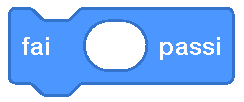
\includegraphics[width=78bp]{img/scratchblocks-cap08/pdf/scratch-faipassi.pdf}\label{credito:scratch-faipassi-1}. Per confrontarlo con gli altri comandi, distinguiamo due modi di indicare uno spostamento:

\begin{itemize}
\item
  \textbf{Movimento relativo}: si indica di quanto modificare la posizione attuale. Con 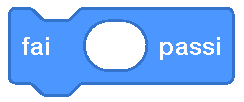
\includegraphics[width=78bp]{img/scratchblocks-cap08/pdf/scratch-faipassi.pdf}\label{credito:scratch-faipassi-2}, lo spostamento dipende anche dalla direzione in cui sta guardando lo sprite: per esempio, 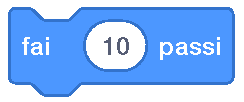
\includegraphics[width=78bp]{img/scratchblocks-cap08/pdf/scratch-fai10.pdf}\label{credito:scratch-fai10-3} fa avanzare lo sprite di 10 passi (cioè 10 unità dello stage), a partire dalla posizione in cui si trova, nella direzione in cui sta guardando. Se, anche partendo dalla stessa posizione, avesse avuto lo sguardo puntato in un'altra direzione, la posizione di arrivo sarebbe stata diversa;
\item
  \textbf{Movimento assoluto}: si indica la posizione da raggiungere tramite le coordinate dello stage. La direzione dello sguardo non influisce e non viene cambiata. Per esempio, il comando 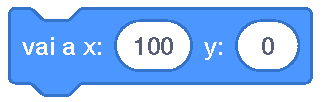
\includegraphics[width=103bp]{img/scratchblocks-cap08/pdf/testo-vai-100-0.pdf}\label{credito:testo-vai-100-0-1}, qualunque sia la posizione di partenza dello sprite e la direzione iniziale verso cui guarda, porta lo sprite nel punto (100, 0) dello stage lasciando invariata la direzione.
\end{itemize}

\begingroup
\manualeimpostazioni
\setlength{\LTleft}{0pt}
\setlength{\LTright}{0pt}
\newcommand{\bloccotabellamovimento}[2]{%
  \manualeimmagini{\includegraphics[width=#1]{#2}}}
\begin{longtable}{|K{\dimexpr0.47\linewidth-2\tabcolsep-1.5\arrayrulewidth\relax}|J{\dimexpr0.53\linewidth-2\tabcolsep-1.5\arrayrulewidth\relax}|}
\arrayrulecolor{guideManualeBordo}
\hline
\manualetitolo{2}{SPOSTAMENTI SCRATCH}
\manualeintestazione
\endfirsthead
\hline
\manualetitolo{2}{SPOSTAMENTI SCRATCH}
\manualeintestazione
\endhead
\bloccotabellamovimento{78bp}{img/scratchblocks-cap08/pdf/scratch-faipassi.pdf}\label{credito:scratch-faipassi-3} & Sposta lo sprite del numero di passi (unità, pixel) indicato, a partire dalla posizione attuale e nella sua direzione corrente. Con un valore negativo si muove nel verso opposto, senza cambiare direzione dello sguardo. \\
\hline
\bloccotabellamovimento{98.5bp}{img/scratchblocks-cap08/pdf/scratch-vai-a.pdf}\label{credito:scratch-vai-a-2} & Porta istantaneamente lo sprite nel punto di coordinate (\emph{x}, \emph{y}), senza cambiarne la direzione. \\
\hline
\bloccotabellamovimento{180bp}{img/scratchblocks-cap08/pdf/scratch-scivola.pdf}\label{credito:scratch-scivola-1} & Porta lo sprite nel punto di coordinate (\emph{x}, \emph{y}) nel tempo indicato, senza cambiarne la direzione. A parità di percorso, più tempo significa minore velocità. \\
\hline
\bloccotabellamovimento{82.5bp}{img/scratchblocks-cap08/pdf/tabella-posizione-xy.pdf}\label{credito:tabella-posizione-xy-1} & Imposta la coordinata \emph{x} oppure \emph{y} al valore indicato, e quindi sposta istantaneamente lo sprite lasciando invariate l'altra coordinata e la direzione. \\
\hline
\bloccotabellamovimento{81bp}{img/scratchblocks-cap08/pdf/tabella-variazione-xy.pdf}\label{credito:tabella-variazione-xy-1} & Aggiunge il valore indicato al valore della coordinata \emph{x} oppure \emph{y} attuale: lo spostamento avviene parallelamente all'asse corrispondente, senza cambiare la direzione dello sprite né dipendere da essa. \\
\hline
\bloccotabellamovimento{131.5bp}{img/scratchblocks-cap08/pdf/scratch-rimbalza.pdf}\label{credito:scratch-rimbalza-1} & Se lo sprite tocca un bordo, si allontana dal bordo
come se avesse colpito una superficie rigida. \\
\hline
\bloccotabellamovimento{159.5bp}{img/scratchblocks-cap08/pdf/scratch-stile-rotazione.pdf}\label{credito:scratch-stile-rotazione-1} & Permette di selezionare lo stile di rotazione: sinistra-destra significa che lo sprite può guardare a sinistra e a
destra, ma non si inclinerà. \\
\hline
\end{longtable}
\manualeripristinacolore
\endgroup




\newpage
\Needspace{10\baselineskip}
\begin{consiglio}[Maestr* si è buggato... non si muove!]

\noindent
\begin{minipage}[t]{0.28\linewidth}
\vspace{0pt}
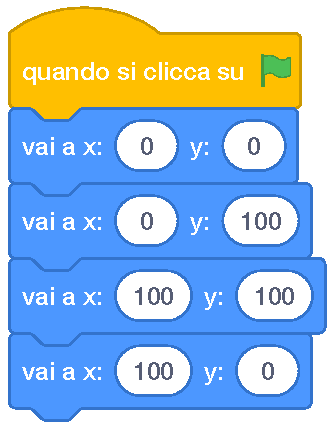
\includegraphics[width=107.5bp]{img/scratchblocks-cap08/pdf/scratch-vai-inutili.pdf}\label{credito:scratch-vai-inutili-1}
\end{minipage}\hfill
\begin{minipage}[t]{0.68\linewidth}
\vspace{0pt}
Può capitare che, anche usando i blocchi di movimento corretti, lo sprite sembri non spostarsi alle coordinate indicate, come nel programma a fianco (provatelo!). In realtà si sta muovendo eccome, ma così velocemente che l'occhio non fa in tempo a percepire il cambiamento. Per questo motivo, dal punto di vista grafico il programma qui a fianco è equivalente al solo ultimo blocco.
\end{minipage}

Per rendere visibile il movimento potete:

\begin{itemize}
  \item inserire un blocco 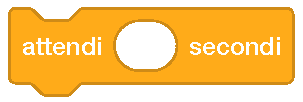
\includegraphics[width=97bp]{img/scratchblocks-cap08/pdf/scratch-attendi.pdf}\label{credito:scratch-attendi-2} tra un movimento e l'altro, così lo sprite farà una piccola pausa prima del passo successivo;
  \item oppure usare il blocco 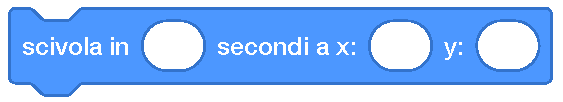
\includegraphics[width=180bp]{img/scratchblocks-cap08/pdf/scratch-scivola.pdf}\label{credito:scratch-scivola-2}, che mostra il percorso sullo stage in modo fluido e chiaro.

\end{itemize}



\end{consiglio}

\begin{consiglio}[Maestr* come faccio ad andare indietro?]

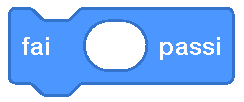
\includegraphics[width=78bp]{img/scratchblocks-cap08/pdf/scratch-faipassi.pdf}\label{credito:scratch-faipassi-4}In Scratch il blocco \textbf{fai \ldots{} passi} fa muovere lo sprite nella direzione in cui sta guardando. Per andare nella direzione opposta non serve un blocco nuovo: basta usare un numero negativo. Per esempio, il valore -10 nel blocco 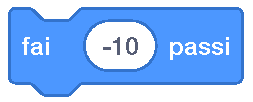
\includegraphics[width=81bp]{img/scratchblocks-cap08/pdf/testo-passi-negativi.pdf}\label{credito:testo-passi-negativi-1} fa muovere lo sprite di 10 passi nel verso opposto a dove sta guardando. Questo è un ottimo momento per far notare a bambini e bambine che anche i numeri con il segno davanti hanno un effetto preciso sul movimento. Non è necessario formalizzare i numeri negativi dal punto di vista matematico: si tratta di sperimentare e osservare cosa succede allo sprite quando si cambia il valore numerico nel blocco.

\end{consiglio}


\section{Attività 6: sperimentare programmi}

\ruoliattivita{\ruoloProgrammatore}

In questa attività alunne e alunni copiano in Scratch alcuni programmi già pronti, per scoprire che effetto hanno.

Per esempio, puoi fornire loro questi programmi:

\begin{center}
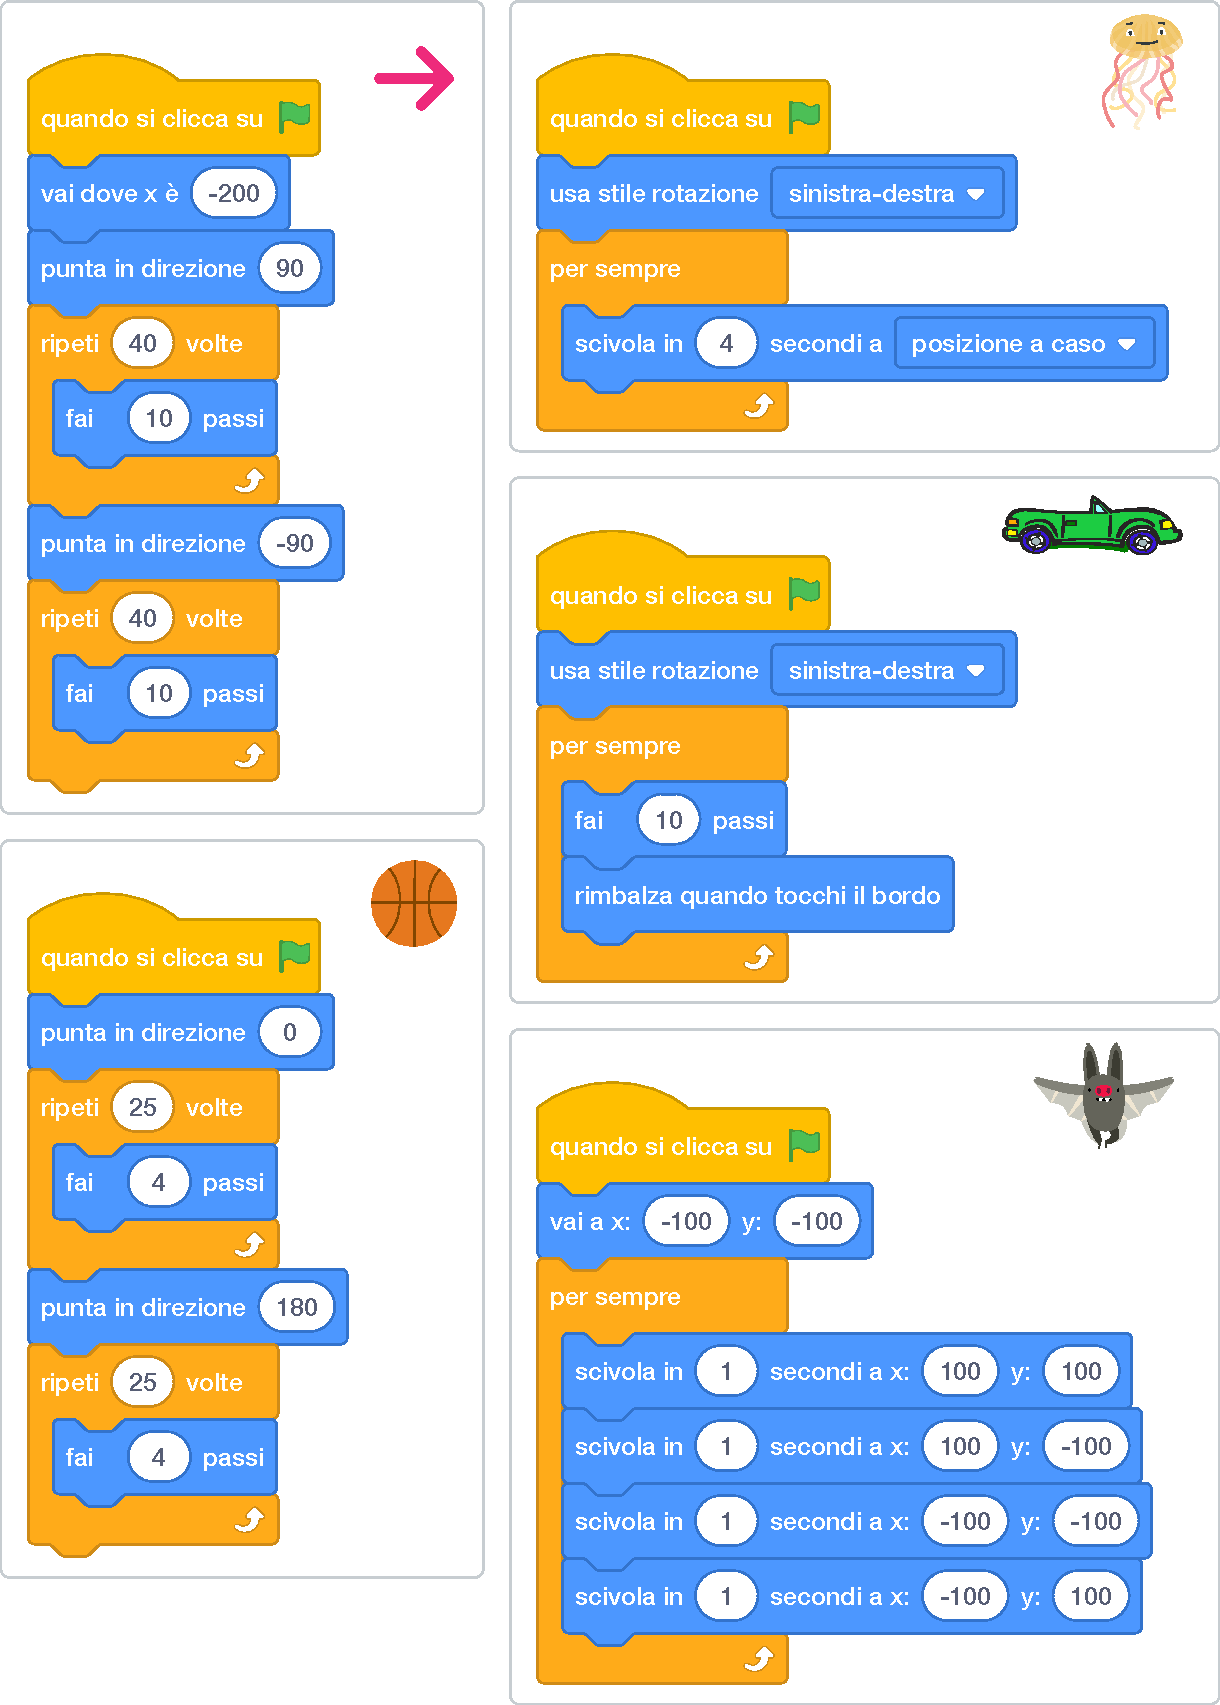
\includegraphics[width=\linewidth]{img/scratchblocks-cap08/pdf/figure-sperimentare-programmi.pdf}\label{credito:figure-sperimentare-programmi-1}
\end{center}


Copiare e provare i programmi già pronti è un modo efficace per imparare a programmare, soprattutto se accompagnati da domande che stimolano la riflessione. Mentre ricostruiscono i blocchi uno alla volta, gli alunni e le alunne osservano cosa succede sullo schermo, fanno ipotesi, notano differenze e scoprono nuovi concetti senza bisogno di spiegazioni astratte. Questo approccio offre la possibilità di:

\begin{itemize}
\item
  imparare osservando cosa fa ogni blocco;
\item
  capire la struttura del programma semplicemente ricreandolo;
\item
  esplorare idee nuove in modo guidato ma creativo;
\item
  aumentare il proprio senso di sicurezza riproducendo un codice che funziona.
\end{itemize}

È un po' come quando si impara a leggere copiando parole: prima si imita, poi si diventa capaci di crearne di nuove. Copiare programmi non è solo utile: è un passo fondamentale per costruire autonomia e padronanza nella programmazione.

Alcuni suggerimenti operativi:

\begin{itemize}
\item
  Dopo aver copiato un programma e prima di eseguirlo, invitate bambini e bambine a rispondere alla domanda: ``Secondo te cosa succederà?''
\item
  Chiedete agli alunni e alle alunne di modificarne un solo elemento: ad esempio un numero, un blocco, un costume o una direzione. Una variazione alla volta aiuta a capire quale blocco produce quale effetto.
\end{itemize}

\section{Attività 7: solo 10 blocchi!}

\ruoliattivita{\ruoloProgrammatore}

Questa sfida riprende l'attività ``10 Blocchi'' della guida \textit{Creative Computing} di \citeauthor{brennan-creative-computing}, disponibile anche nella traduzione italiana (pp.~30--31; \linkbreve{scratchGuida}).

In questa sfida gli alunni e le alunne devono inventare un programma usando soltanto i dieci tipi di blocco proposti di seguito. Ogni tipo deve comparire almeno una volta, ma può essere usato anche più volte. Alcuni blocchi li conoscono già, altri li scopriranno giocando e sperimentando! Aiutate gli alunni a cercare i blocchi nell'Area dei blocchi in base ai colori.

\begin{center}
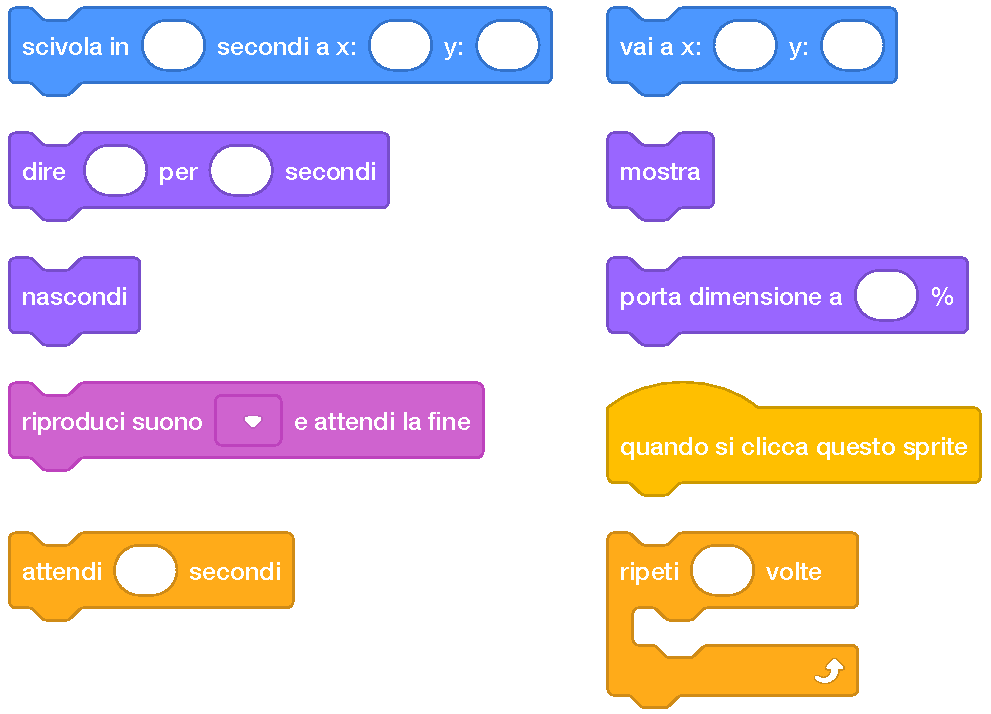
\includegraphics[width=0.92\linewidth]{img/scratchblocks-cap08/pdf/scratch-10blocchi.pdf}\label{credito:scratch-10blocchi-1}
\end{center}


A differenza della ``tela bianca'' di Scratch, che permette di usare subito tutti i comandi disponibili, qui si lavora entro un insieme ristretto di blocchi. Questo non è un limite: anzi, i vincoli diventano un motore per la creatività. Quando le possibilità sono definite, si è spinti a esplorare ogni blocco, anche quelli che normalmente verrebbero ignorati, e a combinarli in modi nuovi.

Per questo tipo di attività, l'insegnante può creare altre sfide scegliendo set diversi di blocchi (per esempio prendendone 7 o 8). L'importante è che i blocchi selezionati permettano comunque di costruire programmi vari e significativi, possibilmente diversi da quelli già realizzati in classe, così da ampliare l'immaginario di ciascuno e stimolare nuove idee.

\section{Bonus: costumi e suoni }\label{bonus-costumi-e-suoni}

\ruoliattivita{\ruoloProgrammatore}

\noindent
\begin{minipage}[c]{0.44\linewidth}
\centering
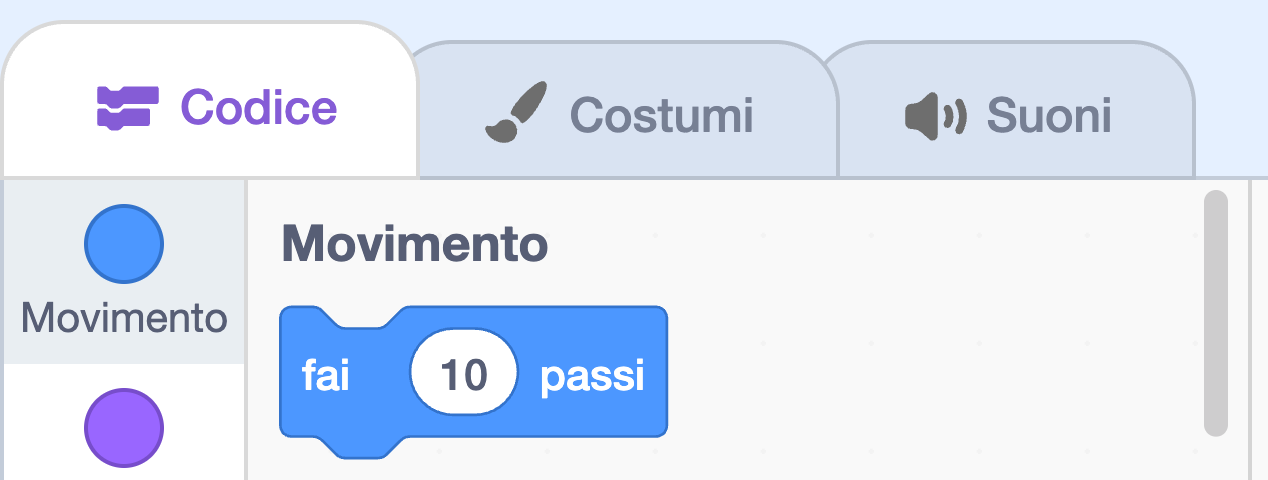
\includegraphics[width=\linewidth]{img/scratch-linguette.png}\label{credito:scratch-linguette-1}
\end{minipage}\hfill
\begin{minipage}[c]{0.52\linewidth}
Per concludere, parliamo di due funzionalità interessanti da presentare in classe: costumi e suoni. Alcuni degli sprite di Scratch hanno a disposizione diversi \textbf{costumi}, cioè immagini alternative con aspetti o posizioni differenti. Allo stesso modo, ogni sprite può essere associato a uno o più \textbf{suoni}, che possono essere riprodotti dalle casse del computer.
\end{minipage}
\par

È possibile vedere costumi e suoni associati allo sprite cliccando sulle linguette a fianco della linguetta codice, in alto sopra l'Area dei blocchi. Per tornare al codice, è sufficiente cliccare sulla linguetta corrispondente. Nella scheda ``Costumi'' è possibile scegliere costumi, disegnarne di nuovi, duplicarli o modificarli. I costumi permettono di trasformare lo sprite in modo creativo, ad esempio cambiando espressione, postura, colori o dettagli del personaggio.

Sono anche uno strumento importante per creare \textbf{animazioni}: alternando due o più costumi e combinandoli con blocchi di movimento, si può simulare l'effetto di un personaggio che cammina, corre o sbatte le ali. Nello sprite dell'ippopotamo, per esempio, esistono due costumi che mostrano le ali in posizioni diverse (su/giù): utilizzando il blocco 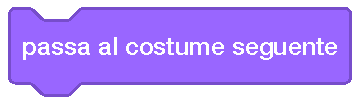
\includegraphics[width=115.5bp]{img/scratchblocks-cap08/pdf/scratch-costume-seguente.pdf}\label{credito:scratch-costume-seguente-1} (\textbf{Aspetto}) dentro una ripetizione per sempre è possibile fare battere le ali al nostro ippopotamo.


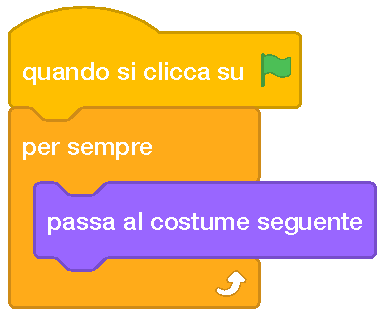
\includegraphics[width=123bp]{img/scratchblocks-cap08/pdf/scratch-ripeti-costume.pdf}\label{credito:scratch-ripeti-costume-1}


\noindent
\begin{minipage}[c]{0.81\linewidth}
Per creare un \textbf{nuovo suono} bisogna premere sull'icona con l'altoparlante e scegliere uno dei modi possibili (dall'alto verso il basso):

\begin{itemize}
\item
  caricare un file audio dal computer;
\item
  far scegliere a Scratch un suono dalla libreria in maniera casuale;
\item
  registrarlo;
\item
  sceglierlo dalla libreria di Scratch.
\end{itemize}
\end{minipage}\hfill
\begin{minipage}[c]{0.15\linewidth}
\centering
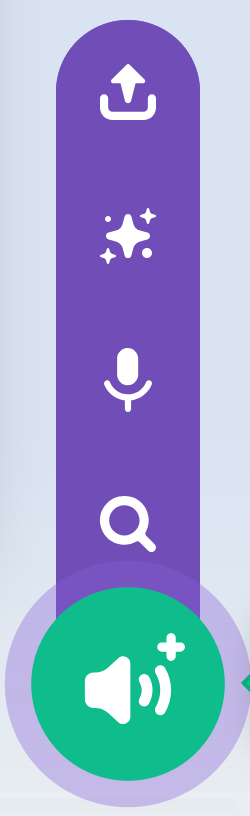
\includegraphics[height=1.4in]{img/scratch-scegli-suono.png}\label{credito:scratch-scegli-suono-1}
\end{minipage}
\par

È poi possibile riprodurre il suono scelto con il blocco 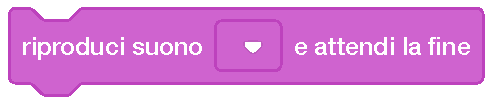
\includegraphics[width=180bp]{img/scratchblocks-cap08/pdf/scratch-suono.pdf}\label{credito:scratch-suono-1} (\textbf{Suono}).



\section{Modalità di lavoro }\label{modalituxe0-di-lavoro-5}

\subsection{Programmazione in coppia }\label{programmazione-in-coppia-1}

Nel Capitolo~\ref{capitolo-7-code.org} abbiamo introdotto la metodologia della programmazione in coppia (\ref{programmazione-in-coppia}), evidenziando i ruoli di \textbf{pilota} e \textbf{navigatore}. Quel modello resta valido anche in Scratch: lavorare in coppia è un potente strumento per favorire attenzione, verbalizzazione, confronto, pianificazione e debugging.

In Scratch però il contesto cambia. Non ci sono puzzle da risolvere, né un pulsante dedicato a tracciare automaticamente il lavoro dei partner. Qui gli alunni e le alunne non si limitano a seguire un percorso guidato: progettano liberamente storie, dialoghi, animazioni e movimenti sullo stage. Questo rende la collaborazione ancora più preziosa, perché richiede decisioni condivise su cosa fare, come farlo e perché. Alcuni consigli per aiutare le coppie a collaborare:

\begin{itemize}
\item
  invitali a discutere e concordare insieme la scena da realizzare prima di iniziare a programmare;
\item
  chiedi al pilota di raccontare le proprie scelte;
\item
  ricorda a ciascuna coppia di scambiarsi i ruoli regolarmente.
\end{itemize}

\subsection{Usa-Modifica-Crea (UMC) }\label{usa-modifica-crea-umc}

Anche in Scratch ritroviamo l'approccio UMC (\ref{usa-modifica-crea}), già introdotto nel Capitolo~\ref{capitolo-7-code.org}: si parte da programmi esistenti, si esplorano piccole modifiche e poi si arriva alla creazione di progetti personali. La logica di fondo resta la stessa, ma in Scratch assume una forma più aperta e creativa.

\begin{itemize}
\item
  \textbf{Usa}: alunni e alunne provano programmi già costruiti dall'insegnante (per esempio animazioni o dialoghi) e osservano che cosa succede sullo stage, senza dover ricostruire tutto da zero.
\item
  \textbf{Modifica}: alunni e alunne cambiano numeri, blocchi, direzioni, costumi o tempi, prima facendo previsioni e poi confrontando previsione e risultato. Anche un singolo cambiamento può trasformare in modo evidente il comportamento dello sprite.
\item
  \textbf{Crea}: grazie alla libertà di movimento nello stage, ai costumi, ai suoni e ai dialoghi, la fase di creazione diventa naturalmente più ampia: ciascuno può progettare qualcosa di unico, non solo una variante del modello di partenza.
\end{itemize}

In Scratch, quindi, l'UMC mantiene la struttura per proporre i concetti, ma si arricchisce di un elemento nuovo: non si risolve un problema dato, si progetta un'idea personale. Questo valorizza il pensiero creativo e la progettazione autentica, mettendo al centro l'immaginazione di alunni e alunne.

\section{Aspetti informatici }\label{aspetti-informatici-4}

In questo capitolo, alunni e alunne continuano a lavorare con un linguaggio di programmazione visuale, ritrovando molti concetti già incontrati con Code.org: \textbf{sintassi} (i blocchi si incastrano solo in certi modi), \textbf{semantica} (ogni blocco ha un significato preciso), \textbf{esecutore meccanico} (lo sprite fa solo ciò che è scritto), \textbf{algoritmi} e \textbf{programmi}, \textbf{sequenza} e \textbf{ripetizioni}, \textbf{parametri} e \textbf{debugging}. La logica di fondo non cambia: un programma è una sequenza di istruzioni che il computer esegue alla lettera.

Quello che cambia è l'ambiente: in Scratch il programmatore deve ragionare non solo su \textbf{cosa} fare, ma anche su \textbf{dove} farlo accadere e su \textbf{come} un personaggio può comportarsi nel tempo. Questo introduce alcune idee nuove e importanti.

\begin{itemize}
\item
  \textbf{Creatività e progettazione libera.} A differenza dei puzzle proposti in Code.org, qui non c'è un obiettivo già definito da raggiungere. Alunni e alunne devono decidere che cosa vogliono ottenere: una scena, un dialogo, un'animazione, una storia, un gioco. L'informatica non è più solo trovare la soluzione corretta a un problema dato, ma immaginare il problema stesso e costruire un percorso per risolverlo. La dimensione creativa non è un'aggiunta estetica: è parte centrale della competenza informatica, perché costringe a fare scelte, a definire scopi e a trasformarli in istruzioni chiare.
\item
  \textbf{Debugging come ricerca del risultato desiderato}. In questo contesto il debugging assume un significato diverso rispetto ai puzzle: non si tratta più soltanto di far funzionare il programma nel modo ``giusto'', ma di capire perché il comportamento osservato è diverso da quello voluto. Bambini e bambine devono confrontare l'idea che avevano con ciò che accade sullo stage, e rivedere il codice fino a ottenere l'effetto desiderato. Questo rende il debugging un processo più aperto e riflessivo, dove si impara dai propri tentativi, invece di inseguire un'unica risposta esatta.
\end{itemize}

\section{Relazione con l'informatica nelle Indicazioni Nazionali 2025 }\label{relazione-con-linformatica-nelle-indicazioni-nazionali-5}

Relativamente alle Indicazioni Nazionali 2025, queste attività contribuiscono allo sviluppo delle seguenti competenze, obiettivi e conoscenze (queste ultime inserite nelle Indicazioni Nazionali 2025 a titolo di esempio, non prescrittive).


\subsubsection{Competenze (alla fine della scuola primaria) nella disciplina Matematica}


\begin{itemize}
\item
  \emph{Scrivere e comprendere semplici programmi, espressi in elementari linguaggi di programmazione a scopo didattico, e valutarne l'adeguatezza rispetto al compito che si vuole automatizzare.}
\end{itemize}


\subsubsection{Competenze (alla fine della scuola primaria) nella disciplina Tecnologia}


\begin{itemize}
\item
  \emph{Sviluppare un atteggiamento positivo nei confronti delle applicazioni informatiche riconoscendone le potenzialità come strumenti di espressione personale nella vita quotidiana.}
\end{itemize}



\subsubsection{Obiettivi (alla fine della terza primaria) nella disciplina Matematica}


\begin{itemize}
\item
  \emph{Scrivere semplici programmi e verificare, mediante la loro esecuzione, se svolgono il compito previsto ed eventualmente correggerli.}
\end{itemize}


\subsubsection{Obiettivi (alla fine della terza primaria) nella disciplina Tecnologia}


\begin{itemize}
\item
  \emph{Creare, selezionare e usare semplici testi o disegni, usando strumenti informatici.}
\end{itemize}



\subsubsection{Conoscenze (scuola primaria) nella disciplina Matematica}


\begin{itemize}
\item
  \emph{Concetto di algoritmo e sua esecuzione rigorosa.} In particolare qui si lavora sulla creazione ed esecuzione di programmi, cioè algoritmi scritti in un linguaggio di programmazione (qui, in particolare, il linguaggio Scratch);
\item
  \emph{Strutture di controllo fondamentali di un linguaggio di programmazione e reazione agli eventi.}
\item
  \emph{Controllo di correttezza dei programmi.}
\end{itemize}

\subsubsection{Conoscenze (scuola primaria) nella disciplina Tecnologia}

\begin{itemize}
\item
  \emph{Creazione e modifica di semplici contenuti digitali e multimediali usando semplici applicazioni informatiche, per raccontare storie o esperienze personali.}
\end{itemize}

\section{Valore costruzionista }\label{valore-costruzionista-5}

In Scratch l'apprendimento non nasce dalla ricerca della ``risposta giusta'', ma dalla costruzione di qualcosa di personale e significativo. Ogni progetto è un artefatto che prende forma nel tempo attraverso tentativi, modifiche e nuove idee. Questo modo di lavorare rispecchia l'idea dell'\textbf{apprendimento creativo}, al centro della spirale proposta da \textcite{resnick-2018}: immaginare → creare → giocare → condividere → riflettere, e di nuovo immaginare:

\begin{itemize}
\item
  \textbf{Immaginare}: ciascuno parte da un'idea propria, per esempio inventando una storia.
\item
  \textbf{Creare}: si traduce l'idea in blocchi di codice, costumi, movimenti e posizioni, scoprendo strumenti nuovi mentre vengono usati.
\item
  \textbf{Giocare}: si esegue il programma e si osserva cosa accade, divertendosi a modificare blocchi, numeri e costumi per vedere nuovi effetti.
\item
  \textbf{Condividere}: ciascuno mostra il proprio lavoro agli altri, facendoglielo provare e ascoltando idee e punti di vista diversi.
\item
  \textbf{Riflettere}: ci si accorge di cosa funziona e cosa no, e si cambia il progetto per migliorarlo o trasformarlo.
\end{itemize}

In classe questo processo appare molto chiaramente: il debugging non serve solo a correggere errori tecnici, ma a chiarire l'intenzione del progetto (``cosa volevo fare davvero?''), e ogni modifica apre possibilità nuove. L'attenzione si sposta dal risultato all'esperienza--una forma di apprendimento attivo che unisce creatività, logica e collaborazione.

\section{Suggerimenti per ulteriori attività}\label{suggerimenti-per-ulteriori-attivituxe0-e-riferimenti-5}

\printbibliography[heading=none,keyword={cap8},category={attivita}]

\begin{rimandiquaderno}
Se possiedi il volume studente \emph{Sulle orme di Milù -- Informatica}
(Mondadori Education, 2026), puoi usare i rimandi seguenti per affiancarlo
alle attività di questo capitolo.\par\smallskip

\begin{itemize}[leftmargin=*,itemsep=5pt,topsep=4pt]
\item \textbf{Benvenuti in Scratch! (Attività 1).} Le schede BENVENUTI IN SCRATCH (pagg.~36--37) accompagnano l'esplorazione dell'interfaccia e si possono tenere aperte mentre si riflette sulla funzione delle diverse aree della schermata.
\item \textbf{Diventa un regista con Scratch! (Attività 2).} Nelle schede DIVENTA UN REGISTA CON SCRATCH (pagg.~38--39) puoi seguire i passi indicati per scegliere un personaggio e fargli pronunciare due o tre frasi con i blocchi ``dire''.
\item \textbf{Dialogo tra due personaggi (Attività 3).} Nella scheda DIALOGO TRA DUE PERSONAGGI (pag.~40) è proposto il dialogo tra ippopotamo e ragnetto descritto nella guida.
\item \textbf{Movimenti precisi (Attività 4).} Nelle schede MOVIMENTI PRECISI, i box di pag.~42 guidano l'esplorazione delle proprietà dimensione e direzione; le attività di pag.~43 guidano l'esplorazione della posizione dello sprite.
\item \textbf{Posizionare un personaggio (Attività 5).} Nella scheda POSIZIONARE UN PERSONAGGIO (pag.~44) è proposto un programma analogo a quello della guida, da copiare passo per passo, per sperimentare diverse coordinate di partenza. In ALTRI BLOCCHI DI MOVIMENTO (pag.~45) si lavora sulle direzioni.
\item \textbf{Sperimentare programmi (Attività 6).} Nella scheda SPERIMENTARE PROGRAMMI (pag.~46) sono disponibili programmi già pronti da copiare in Scratch per scoprirne l'effetto.
\item \textbf{Solo 10 blocchi! (Attività 7).} Nella scheda SOLO 8 BLOCCHI! (pag.~47) è proposta una sfida analoga a quella dei 10 blocchi presentata nella guida.
\end{itemize}
\end{rimandiquaderno}

\section{Riferimenti}\label{riferimenti-cap8}

\printbibliography[heading=none,keyword={cap8},notcategory={attivita}]
